\documentclass[UTF8,a4paper,12pt]{ctexbook} 

\usepackage{graphicx}%学习插入图
\usepackage{verbatim}%学习注释多行
\usepackage{booktabs}%表格
\usepackage{longtable} 
\usepackage{geometry}%图片
\usepackage{amsmath}
\usepackage{amssymb}
\usepackage{listings}%代码
\usepackage{xcolor}  %颜色
\usepackage{enumitem}%列表格式
\setenumerate[1]{itemsep=0pt,partopsep=0pt,parsep=\parskip,topsep=5pt}
\setitemize[1]{itemsep=0pt,partopsep=0pt,parsep=\parskip,topsep=5pt}
\setdescription{itemsep=0pt,partopsep=0pt,parsep=\parskip,topsep=5pt}

\usepackage{tcolorbox}
\usepackage{algorithm}  %format of the algorithm
\usepackage{algorithmic}%format of the algorithm
\usepackage{multirow}   %multirow for format of table
\usepackage{tabularx} 	%表格排版格式控制
\usepackage{array}	%表格排版格式控制
\usepackage{hyperref}
\usepackage{dirtree}
\setmainfont{Times New Roman}
\graphicspath{{figure/}}
\CTEXsetup[format+={\flushleft}]{section}
%%%% 下面的命令添加新字体 %%%%%


%%%%%% 设置字号 %%%%%%
\newcommand{\chuhao}{\fontsize{42pt}{\baselineskip}\selectfont}
\newcommand{\xiaochuhao}{\fontsize{36pt}{\baselineskip}\selectfont}
\newcommand{\yihao}{\fontsize{28pt}{\baselineskip}\selectfont}
\newcommand{\erhao}{\fontsize{21pt}{\baselineskip}\selectfont}
\newcommand{\xiaoerhao}{\fontsize{18pt}{\baselineskip}\selectfont}
\newcommand{\sanhao}{\fontsize{15.75pt}{\baselineskip}\selectfont}
\newcommand{\sihao}{\fontsize{14pt}{\baselineskip}\selectfont}
\newcommand{\xiaosihao}{\fontsize{12pt}{\baselineskip}\selectfont}
\newcommand{\wuhao}{\fontsize{10.5pt}{\baselineskip}\selectfont}
\newcommand{\xiaowuhao}{\fontsize{9pt}{\baselineskip}\selectfont}
\newcommand{\liuhao}{\fontsize{7.875pt}{\baselineskip}\selectfont}
\newcommand{\qihao}{\fontsize{5.25pt}{\baselineskip}\selectfont}

%%%% 段落首行缩进两个字 %%%%
\makeatletter
\let\@afterindentfalse\@afterindenttrue
\@afterindenttrue
\makeatother
\setlength{\parindent}{2em}  %中文缩进两个汉字位


%%%% 下面的命令重定义页面边距,使其符合中文刊物习惯 %%%%
\addtolength{\topmargin}{-54pt}
\setlength{\oddsidemargin}{0.63cm}  % 3.17cm - 1 inch
\setlength{\evensidemargin}{\oddsidemargin}
\setlength{\textwidth}{14.66cm}
\setlength{\textheight}{24.00cm}    % 24.62

%%%% 下面的命令设置行间距与段落间距 %%%%
\linespread{1.4}
\setlength{\parskip}{0.5\baselineskip}

%%%% 下面的命令定义图表、算法、公式 %%%%
\newcommand{\EQ}[1]{$\textbf{EQ:}#1\ $}
\newcommand{\ALGORITHM}[1]{$\textbf{Algorithm:}#1\ $}
\newcommand{\Figure}[1]{$\textbf{Figure }#1\ $}

%%%% 下面命令改变图表下标题的前缀 %%%%% 如:图-1、Fig-1
\renewcommand{\figurename}{Fig}

\geometry{left=1.6cm,right=1.8cm,top=2cm,bottom=1.7cm} %设置文章宽度

\pagestyle{plain} 		  %设置页面布局

%代码效果定义
\definecolor{mygreen}{rgb}{0,0.6,0}
\definecolor{mygray}{rgb}{0.5,0.5,0.5}
\definecolor{mymauve}{rgb}{0.58,0,0.82}
\lstset{ %
	backgroundcolor=\color{white},   % choose the background color
	basicstyle=\footnotesize\ttfamily,        % size of fonts used for the code
	columns=fullflexible,
	breaklines=true,                 % automatic line breaking only at whitespace
	captionpos=b,                    % sets the caption-position to bottom
	tabsize=4,
	commentstyle=\color{mygreen},    % comment style
	escapeinside={\%*}{*)},          % if you want to add LaTeX within your code
	keywordstyle=\color{blue},       % keyword style
	stringstyle=\color{mymauve}\ttfamily,     % string literal style
	frame=single,					%tb top and bottom; L left double line
	xleftmargin=.06\textwidth, 
	%xrightmargin=.1\textwidth,
	rulesepcolor=\color{red!20!green!20!blue!20},
	% identifierstyle=\color{red},
	language=c++,
}
\setcounter{tocdepth}{3}	
\author{\kaishu 郑华}
\title{\heiti Linux 学习笔记}

\begin{document}          %正文排版开始
 	\maketitle
 	\tableofcontents
 	
 \chapter{Linux 基本知识} 
	 \section{基本技能}
		 正如你所见,Linux发行版并非Linux,Linux仅是指操作系统的内核。

		 \subsection{推荐的发行版}
		 \begin{itemize}
			 \item UBUNTU 适合纯菜鸟,追求稳定的官方支持,对系统稳定性要求较弱,喜欢最新应用,相对来说不太喜欢折腾的开发者。
			 \item Debian,相对UBUNTU难很多的发行版,突出特点是稳定与容易使用的包管理系统,缺点是企业支持不足,为社区开发驱动。
			 \item Arch,追逐时尚的开发者的首选,优点是包更新相当快,无缝升级,一次安装基本可以一直运作下去,没有如UBUNTU那样的版本概念,说的专业点叫滚动升级,保持你的系统一定是最新的。缺点显然易见,不稳定。同时安装配置相对Debian再麻烦点。
			 \item Gentoo,相对Arch再难点,考验使用者的综合水平,从系统安装到微调,内核编译都亲历亲为,是高手及黑客显示自己技术手段,按需配置符合自己要求的系统的首选。
			 \item Slackware与Gentoo类似。
			 \item CentOS,社区维护的RedHat的复刻版本,完全使用RedHat的源码重新编译生成,与RedHat的兼容性在理论上来说是最好的。如果你专注于Linux服务器,如网络管理,架站,那么CentOS是你的选择。
			 \item LFS,终极黑客显摆工具,完全从源代码安装,编译系统。安装前你得到的只有一份文档,你要做的就是照文档你的说明,一步步,一条条命令,一个个软件包的去构建你的Linux,完全由你自己控制,想要什么就是什么。如果你做出了LFS,证明你的Linux功底已经相当不错,如果你能拿LFS文档活学活用,再将Linux从源代码开始移植到嵌入式系统,我敢说中国的企业你可以混的很好。 
		\end{itemize}
		
		\subsection{Linux基础}
			你得挑一个适合你的系统,然后在虚拟机安装它,开始使用它。 如果你想快速学会Linux,我有一个建议就是\textbf{忘记图形界面},不要想图形界面能不能提供你问题的答案, \textbf{而是满世界的去找,去问,如何用命令行解决你的问题}。
			
			在这个过程中,你最好能将Linux的命令掌握的不错,起码常用的命令得知道,同时建立了自己的知识库, 里面是你积累的各项知识。
		
		\subsection{Linux 平台C++ 开发}
			你需要学习的是Linux平台的C/C++开发,同时还有Bash脚本编程,如果你对Java兴趣很深还有Java。 同样,建议你抛弃掉图形界面的IDE,从VIM开始,为什么是VIM,而不是Emacs, 我无意挑起编辑器大战,但我觉得VIM适合初学者,适合手比较笨,脑袋比较慢的开发者。 Emacs的键位太多,太复杂,我很畏惧。然后是GCC,Make,Eclipse(Java,C++或者)。
			
			虽然将C++列在了Eclipse中,但我并不推荐用IDE开发C++,因为这不是Linux的文化, 容易让你忽略一些你应该注意的问题。 IDE让你变懒,懒得跟猪一样。如果你对程序调试,测试工作很感兴趣,\textbf{GDB也得学的很好}, 如果不是GDB也是必修课。这是开发的第一步,注意我并没有提过一句Linux系统API的内容, 这个阶段也不要关心这个。你要做的就是积累经验,在Linux平台的开发经验。
			
			我推荐的书如下:C语言程序设计。 C语言,白皮书当然更好。 C++推荐 C++ Primer Plus, Java我不喜欢,就不推荐了,附一个别人的书单:java 入门书籍。 工具方面推荐\textbf{VIM的官方手册},\textbf{GCC中文文档},\textbf{GDB中文文档},\textbf{GNU开源软件开发指导}(电子书), 汇编语言程序设计(让你对库,链接,内嵌汇编,编译器优化选项有初步了解,不必深度)。
			
			如果你这个阶段过不了就不必往下做了,这是底线,最基础的基础,否则离开,不要霍霍Linux开发。 不专业的Linux开发者作出的程序是与Linux文化或UNIX文化相背的,程序是走不远的, 不可能像Bash,VIM这些神品一样。 所以做不好干脆离开。
		
		\subsection{UNIX环境高级编程}
			UNIX环境高级编程堪称神作,经典中的经典。
			
			接下来进入Linux系统编程,不二选择,\textbf{APUE,UNIX环境高级编程},一遍一遍的看, 看10遍都嫌少,如果你可以在大学将这本书翻烂,里面的内容都实践过,有作品,你口头表达能力够强, 你可以在面试时说服所有的考官。
			
			(可能有点夸张,但APUE绝对是圣经一般的读物,即使是Windows程序员也从其中汲取养分, Google创始人的案头书籍,扎尔伯克的床头读物。)
			
			这本书看完后你会对Linux系统编程有相当的了解,知道Linux与Windows平台间开发的差异在哪? 它们的优缺点在哪?我的总结如下:做Windows平台开发,很苦,微软的系统API总在扩容, 想使用最新潮,最高效的功能,最适合当前流行系统的功能你必须时刻学习。 Linux不是,Linux系统的核心API就100来个,记忆力好完全可以背下来。 而且经久不变,为什么不变,因为要同UNIX兼容,符合POSIX标准。 所以Linux平台的开发大多是专注于底层的或服务器编程。
			
			这是其优点,当然图形是Linux的软肋,但我站在一个开发者的角度,我无所谓,因为命令行我也可以适应, 如果有更好的图形界面我就当作恩赐吧。另外,Windows闭源,系统做了什么你更本不知道, 永远被微软牵着鼻子跑,想想如果微软说Win8不支持QQ,那腾讯不得哭死。 而Linux完全开源,你不喜欢,可以自己改,只要你技术够。
			
			另外,Windows虽然使用的人多,但使用场合单一,专注与桌面。 而Linux在各个方面都有发展,尤其在云计算,服务器软件,嵌入式领域, 企业级应用上有广大前景,而且兼容性一流,由于支持POSIX可以无缝的运行在UNIX系统之上, 不管是苹果的Mac还是IBM的AS400系列,都是完全支持的。 另外,Linux的开发环境支持也绝对是一流的,不管是C/C++,Java,Bash,Python,PHP,Javascript,就连C\#也支持。而微软除Visual Stdio套件以外,都不怎么友好,不是吗?
			
			如果你看完APUE的感触有很多,希望验证你的某些想法或经验,推荐UNIX程序设计艺术, 世界顶级黑客将同你分享他的看法。

	\section{方向选择}			
		\subsection{网络方向}
			服务器软件编写及\textbf{高性能的并发程序}编写
			
			现在是时候做分流了。 大体上我分为四个方向:网络,图形,嵌入式,设备驱动。
			
			如果选择网络,再细分,我对其他的不是他熟悉,只说服务器软件编写及高性能的并发程序编写吧。 相对来说这是网络编程中技术含量最高的,也是底层的。 需要很多的经验,看很多的书,做很多的项目。
			
			我的看法是以下面的顺序来看书:
			\begin{enumerate}
				\item APUE再深读 – 尤其是进程,线程,IPC,套接字
				\item 多核程序设计 - Pthread一定得吃透了,你很NB
				\item UNIX网络编程 – 卷一,卷二
				\item TCP/IP网络详解 – 卷一 再看上面两本书时就该看了
				\item TCP/IP 网络详解 – 卷二 我觉得看到卷二就差不多了,当然卷三看了更好,努力,争取看了
				\item Lighttpd源代码 - 这个服务器也很有名了
				\item Nginx源代码 – 相较于Apache,Nginx的源码较少,如果能看个大致,很NB。看源代码主要是要学习里面的套接字编程及并发控制,想想都激动。如果你有这些本事,可以试着往暴雪投简历,为他们写服务器后台,想一想全球的魔兽都运行在你的服务器软件上。
				\item Linux内核 TCP/IP协议栈 – 深入了解TCP/IP的实现
			\end{enumerate}
			
			如果你还喜欢驱动程序设计,可以看看更底层的协议,如链路层的,写什么路由器,网卡, 网络设备的驱动及嵌入式系统软件应该也不成问题了。
			
			当然一般的网络公司,就算百度级别的也该毫不犹豫的雇用你。 只是看后面这些书需要时间与经验,所以35岁以前办到吧!跳槽到给你未来的地方!
			
		\subsection{图形方向}我觉得图形方向也是很有前途的,以下几个方面。
			\begin{enumerate}
				\item Opengl的工业及游戏开发,国外较成熟。
				\item 影视动画特效,如皮克斯,也是国外较成熟。
				\item GPU计算技术,可以应用在浏览器网页渲染上,GPU计算资源利用上,由于开源的原因,有很多的文档程序可以参考。如果能进火狐开发,或google做浏览器开发,应该会很好 。
			\end{enumerate}
			
		\subsection{嵌入式方向}嵌入式方向没说的,Linux很重要。
			
			掌握多个架构,不仅X86的,ARM的,单片机什么的也必须得懂。 硬件不懂我预见你会死在半路上,我也想走嵌入式方向,但我觉得就学校教授嵌入式的方法, 我连学电子的那帮学生都竞争不过。 奉劝大家,一定得懂硬件再去做,如果走到嵌入式应用开发,只能祝你好运, 不要碰上像Nokia,Hp这样的公司,否则你会很惨的。
			
		\subsection{驱动程序设计}	
			软件开发周期是很长的,硬件不同,很快。 每个月诞生那么多的新硬件,如何让他们在Linux上工作起来,这是你的工作。 由于Linux的兼容性很好,如果不是太低层的驱动,基本C语言就可以搞定,系统架构的影响不大, 因为有系统支持,你可能做些许更改就可以在ARM上使用PC的硬件了, 所以做硬件驱动开发不像嵌入式,对硬件知识的要求很高。
			
			可以从事的方向也很多,如家电啊,特别是如索尼,日立,希捷,富士康这样的厂子,很稀缺的。
		
	\section{硬件设备}
			在linux 系统中,每个设备都被当成一个文件来对待,如图\ref{Name_linux}。
			\begin{table}[H]
				\centering
				\begin{tabular}{p{8cm}<{\centering}|p{5cm}<{\centering}}
					\toprule[1.5pt]
						设备 &  设备在linux 中的文件名 \\
					\midrule
						SATA/USB硬盘/U盘 &  /dev/sd[a-p] \\
						当前鼠标 &  /dev/mouse \\
					\bottomrule[1.5pt]
				\end{tabular}
				\caption{设备文件名}
				\label{Name_linux}
			\end{table}
		\section{磁盘分区知识}
			 磁盘分区是使用分区编辑器(\verb|partition editor|) \textbf{在磁盘上}\textit{划分几个}\textbf{逻辑部分}。碟片一旦划分数个分区(\verb|Partition|),不同类的目录与文件可以存储进不同的分区。
			 
			 \subsection{分区类型}
				 \dirtree{%
					.1 分区结构.
					.2 主分区.
					.2 *主分区.
					.2 *主分区.
					.2 !扩展分区(不能直接放入数据).
					.3 逻辑分区1.
					.3 逻辑分区2.
				 }
				 \subparagraph{主分区}
					 最多有4个,主分区中不能再划分其他类型的分区,因此每个\textbf{主分区}都相当于\textbf{一个逻辑磁盘}(在这一点上主分区和逻辑分区很相似,但主分区是直接在硬盘上划分的,逻辑分区则必须建立于扩展分区中)
					 
				 \subparagraph{扩展分区}
					 最多只有1个,在使用MBR(主引导分区记录)方式下 \textbf{主分区与扩展分区最多只能有4个},而且扩展分区不能写入数据,只能包含逻辑分区
				
				\subparagraph{分区设备文件名}	 
					\verb|/dev/sda+数字| -> 磁盘号+逻辑分区编号
					
					\begin{figure}
						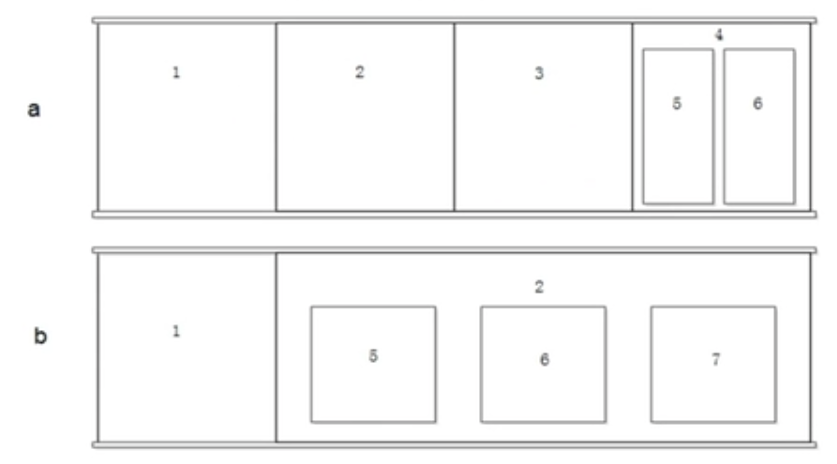
\includegraphics[scale = 0.5]{Fenqu.png}
						\caption{分区设备名表示}
					\end{figure}
						\begin{itemize}[itemindent = 1em]
							\item 扩展分区编号 只能从4开始
						\end{itemize}
						
			\subsection{挂载}
				有了分区,还需要为其分配盘符,这个分配盘符的过程叫做挂载,即给分区盘符(C D E), \textbf{使得系统能够识别不同分区}。
			
				\paragraph{推荐系统分区结构}\verb|->|
					\dirtree{%
						.1 磁盘. 
						.2 /boot.
						.2 /home.
						.2 /.
						.2 sawp.						
					}
				\subparagraph{必须分区}
					\begin{itemize}[itemindent = 1em]
						\item \verb|/| 根分区
						\item \verb|swap| swap分区(交换分区,内存的两倍,不超过2G)
					\end{itemize}
					
				\subparagraph{推荐分区}\verb|/boot| (启动分区,200MB)
				
				
				
			\subsection{GUID}
	\section{裸机装机必备软件及技巧}
		\subparagraph{vim}必备,要么你修改配置文档都是个问题。
			通过wifi 先将基本的vim 搞定。
			
			\verb|sudo apt-get install vim|
			
			编程相关的插件到后续再安装。
			
		\subparagraph{网络配置}有网才能工作
			
			1.ln -s 创建快捷命令
			
			2.1配置IP(一般不动)
			\begin{itemize}[itemindent = 1em]
				\item \verb|vim /etc/network/interfaces|
				\item 根据情况确定用动态IP 还是静态IP 
				\begin{lstlisting}
#动态IP 
	auto eth0
	iface eth0 inet dhcp
	
#静态IP
	auto eth0
	iface eth0 inet static
	address xx.xx.xx.xx
	netmask xx.xx.xx.xx
	gateway xx.xx.xx.xx
				\end{lstlisting}
			\end{itemize}
			
			2.2配置DNS
			\begin{itemize}[itemindent = 1em]
				\item \verb|sudo vi /etc/resolv.conf|
				\item 添加\verb|nameserver 8.8.8.8 或 8.8.4.4|
				\item 重启网络:
				
				\verb|service networking restart|
				
				\verb|sudo /etc/init.d/networking restart|
			\end{itemize}
			
		\subparagraph{更新源}使用国内阿里云镜像,更快速度。

		\subparagraph{输入法}
			\begin{enumerate}[itemindent = 2em]
				\item \verb|sudo apt-get update|
				\item \verb|sudo apt-get install fcitx-googlepinyin|
				\item 注销或重启
				\item 找标题栏中的小企鹅,点开找配置fcitx
				\item 点\verb|+|,取消选中only.查找Google-pinyin
			\end{enumerate}	
					
		\subparagraph{文本工具Texlive与Texstudio}
		
		\subparagraph{git}	
		
		\subparagraph{网易云音乐}有音乐工作才有动力
			\begin{enumerate}[itemindent = 2em]
				\item 官网下载deb
				\item \verb|sudo dpkg -i ~/Downloads/xx.deb|
				\item 出现错误时\verb|sudo apt install -f|
				\item 再次运行安装命令
			\end{enumerate} 
		
		\subparagraph{vim 插件安装}
			\url{http://blog.csdn.net/lhf_tiger/article/details/7216500}
			
			\begin{enumerate}
				\item \verb|Ctags|:
					\verb|sudo apt-get install ctags|
					
					进入目录中
					\verb|ctags -R|
					
					
				\item \verb|Cscope|:
					\url{http://blog.csdn.net/av_geek/article/details/47976981}	
					
					\verb|sudo apt-get install cscope|
					
					\begin{itemize}
						\item 进入项目主目录 \verb|find . -name "*.h" -o -name "*.cc">cscope.files|
						\item 执行 \verb|cscope -bkq -i cscope.files|
						\item 执行 \verb|ctags -R|
						\item 进入要编辑的文件中\verb|:cs add cscope.out|
						\item 然后执行相应的命令 \verb@:cs find c|d|e|f|g|i|s|t name@
					\end{itemize}
			\end{enumerate}
		
 \chapter{命令相关}
	 命令格式:$$\verb|命令  [-选项]  [参数]|$$
	 
	 \begin{enumerate}[itemindent = 1em]
	 	\item 个别命令不遵循此格式
	 	\item 当有多个选项时,可以写在一起 \verb|ls -la 等价于 ls -l -a|
	 	\item 简化选项与完整选项 \verb|-a 等价于 --all|
	 \end{enumerate}
	\section{Linux系统} 
		\paragraph{X windows 与 Console}
			\begin{itemize}[itemindent = 1em]
				\item \verb|ctrl + alt + F1~F6|:Console 终端模式
				\item \verb|ctrl + alt + F7|:图形模式界面
			\end{itemize}
		
		\paragraph{目录结构}linux 目录如表\ref{mulu}所示。
			\begin{table}
				\caption{Linux 目录详解}
				\label{mulu}
				\begin{longtable}{l|m{14cm}}
					\hline
					目录 	   	   & 存放的内容类别\\
					\hline
							\verb|/ |   		&	文件系统的入口,\textbf{最高一级目录}			\\ 
							\verb|/bin| 		&	存放\textbf{系统命令}的目录,\textbf{普通用户和超级用户都可以执行}。不过放在/bin 下的命令\textbf{在单用户模式(安全模式)下也可以执行}\\
							\verb|/sbin|		&	保存和\textbf{系统环境设置}相关的命令,\textbf{只有超级用户}可以使用这些命令进行系统环境设置,部分命令可以被普通用户查看\\
							\verb|/usr/bin| 	&	存放\textbf{系统命令}的目录,\textbf{普通用户和超级用户都可以执行},这些命运与启动无关,不能在单用户模式下运行。\\
							\verb|/usr/sbin|	&	存放\textbf{根文件系统不必要的系统管理}命令,例如多数服务程序,\textbf{只有超级用户}可以使用。/sbin 目录只用超级用户可以使用,/bin 目录存放的命令都可以使用。\\
		
							\verb|/dev|		&	\textbf{设备文件存储目录},是Linux文件系统的一个闪亮的特性 - 所有对象都是文件或目录。仔细观察这个目录你会发现hda1, hda2等, 它们代表系统主硬盘的不同分区。			\\
							\verb|/etc|		&	存放系统程序或者一般工具的\textbf{配置文件}			\\
							
							\verb|/lib|		&	库文件存放目录这里包含了\textbf{系统程序所需要的所有共享库文件},类似于 Windows 的共享库 DLL 文件。			\\
							\verb|/lost+found|	&	在ext2或ext3文件系统中,\textit{当系统意外崩溃或机器意外关机},而\textbf{产生一些文件碎片放在这里}			\\
							\verb|/mnt|		&	这个目录一般是用于\textbf{存放挂载储存设备的挂载目录}的,比如有cdrom 等目录。有时我们可以把让系统开机自动挂载文件系统,把挂载点放在这里也是可以的。比如光驱可以挂载到/mnt/cdrom 			\\
							\verb|/opt|		&	表示的是可选择的意思,\textbf{有些软件包也会被安装在这里,也就是自定义软件包}\\
							\verb|/proc|		&	/proc目录是伪装的文件系统proc的挂载目录,proc并不是真正的文件系统。这个目录本身是一个“虚拟文件系统(virtual filesystem)”喔!他放置的数据都是在内存当中, 例如系统核心、行程信息(process)、周边设备的状态及网络状态等等。因为这个目录下的数据都是在内存当中, 所以本身不占任何硬盘空间啊!\\
							\verb|/tmp|		&	临时文件目录,每次开机会清空该目录。			\\
							\verb|/usr|		& (Unix Software Resources)	这个是\textbf{系统相关第三方程序存放目录},比如命令、帮助文件等。这个目录下有很多的文件和目录。			\\
							\verb|/var |		&	这个目录的内容是经常变动的,如/var/log 系统日志存放,分析日志要看这个目录的东西\\
						\hline
				\end{longtable}
			\end{table}
			\paragraph{PATH}
				当执行一个指令(ls)的时候,系统会依照\verb|$PATH|的设置去每个\verb|$PATH|定义的目录下搜寻文件名为(ls)的可执行文件,如果在\verb|$PATH|定义的目录中含有多个文件名为(ls)的可执行文件,那么先搜寻到的同名指令先被执行。
				
				如果命令不在\verb|$PATH|指定路径下时,单纯敲击指令名称是不会执行的,有以下两种方法可以执行该指令
					\begin{enumerate}
						\item 使用绝对路径或相对路径指定命令 \verb|./ls| 或 \verb|/root/ls|
						\item 将目标目录添加到\verb|PATH|中 \verb|PATH = "${PATH}:/root"|
					\end{enumerate}
			
			\paragraph{用户配置}
				\begin{itemize}
					\item  \verb|~/.bash_profile|
					
						每个用户都可\textit{使用该文件输入}\textbf{专用于自己使用的shell}\textit{信息},\underline{当用户登录时},该文件仅仅执行一次!默认情况下,他设置一些环境变量,执行用户的\verb|.bashrc|文件. 此文件类似于\verb|/etc/profile|,也是需要需要重启才会生效,\verb|~/.bash_profile|\textbf{只对当前用户生效}。
					\item  \verb|~/.bashrc|
						
						该文件包含\textbf{专用于你的bash shell的bash信息},\textit{当登录时以及每次\underline{打开新的shell时},该文件被读取}.(每个用户都有一个\verb|.bashrc|文件,在用户目录下) 此文件类似于\verb|/etc/bashrc|,\textbf{不需要重启生效,重新打开一个bash即可生效}, 但\verb|~/.bashrc|只对当前用户新打开的bash生效。
						
					\item  \verb|/etc/profile|
					
						\verb|/etc/profile|对所有用户生效
					
					\item  \verb|/etc/bashrc|
					
						\verb|/etc/bashrc|对所有用户新打开的bash都生效
				\end{itemize}
			
			\paragraph{交换区} 在内存小于2G的情况下,交换分区\textbf{应为内存的2倍},超过2G的话,交换分区为\textbf{物理内存加上2G}	
			
			\paragraph{符号链接}符号链接又叫软链接,是一类特殊的文件,这个文件包含了\textbf{另一个文件的路径名}
			
			\paragraph{开关机}
				先关服务,再关机
				
				服务器不能关机,只能重启,因为一般都在远程。
				
				\begin{itemize}[itemindent = 1em]
					\item \verb|shutdown -r 20:30|:在20:30 重启
						\begin{enumerate}
							\item \verb|-c|:取消前一个关机命令
							\item \verb|-h|:关机 
							\item \verb|-r|:重启
						\end{enumerate}
					\item \verb|poweroff|
					\item \verb|init 0|
				\end{itemize}
				
			\paragraph{重启}
					\begin{itemize}[itemindent = 1em]
						\item \verb|shutdown -r now|
						\item \verb|reboot|
						\item \verb|init 6|
					\end{itemize}
					
			\paragraph{系统运行级别}\verb|cat /etc/inittab |可以查看运行级别的含义。
					\begin{itemize}[itemindent = 1em]
						\item 0:\textbf{关机}
						\item 1:单用户\verb|-> 安全模式,附加程序构件不运行|
						\item 2:【命令行】不完全多用户,不含NFS服务
						\item 3:【命令行】完全多用户
						\item 4:未分配
						\item 5:【图形界面】
						\item 6:\textbf{重启}
					\end{itemize}
				
				查询当前运行级别:\verb|runlevel|
				
				运行某级别:\verb|init x|
	
	\section{导航命令}
		\paragraph{pwd}Print Working Directory 打印当前工作目录,即当前所处位置的绝对路径
		
			\verb|-P|:显示出确实的路径,而非使用链接\verb|link|路径。
			
			\begin{figure}[h]
				\centering
				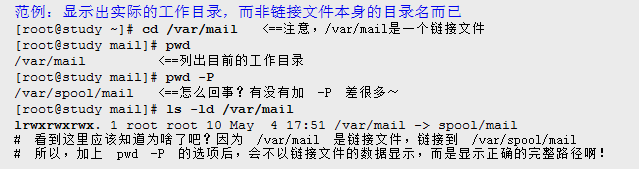
\includegraphics[scale=0.7]{figure/pwd.png}
				\caption{pwd -P 选项示例}
			\end{figure}
		
		\paragraph{cd}改变当前工作目录
			\begin{itemize}[itemindent = 1em]
				\item 绝对路径: 从根目录 / 开始
				\item 相对路径: 从当前位置开始,. 表示当前目录,.. 表示上级目录
				\item \verb|cd ~| || \verb|cd  |: 进入当前用户家目录
				\item \verb|cd - |: 进入上次目录
				\item \verb|cd .. |: 进入上一级目录
				\item \verb|cd . |: 进入当前目录
			\end{itemize}
			
		\paragraph{ls}列出目录内容
			\begin{itemize}[itemindent = 1em]
				\item 所在路径:\verb|/bin/ls|
				\item 执行权限:所有用户
			\end{itemize}
			\begin{table}[H]
				\centering
				\caption{\textbf{ls }参数说明}
				\begin{longtable}{c|c|m{10cm}}
					\toprule[1.5pt]
					简化选项 & 完整选项 & 意义\\
					\midrule
					\verb|-a|  & \verb|--all| & 列出所有文件,包括以点号开头的文件,这些文件通常是不列出来的(比如隐藏的文件)\\
					\verb|-d|  & \verb|--directory| & 查看目录的详细信息,而不是目录里的内容\\
					\verb|-F|  & \verb|--classify|  & 如果名字是目录,则会加上一个斜杠\\
					\verb|-l|  & 			  & 使用长格式显示结果\\
					\verb|-i|  &			  & \verb|–inode| 印出每个文件的\verb|inode|号\\
					\verb|-r|  & \verb|--reverse|   & 以相反的顺序显示结果\\
					\verb|-S|  & 			  & 按照文件的大小对结果进行排序\\
					\verb|-t|  &			  & 按照文件的修改时间排序\\
					\verb|--color|  	& 	\verb|={never, auto, always}|			  & 结果颜色选项\\
					\verb|--full-time|  &	\verb| |		 						  & 完整呈现结果的最后修改时间 \\
					\bottomrule[1.5pt]
				\end{longtable}
			\end{table}
				
	\section{操作文件和目录}
		\subsection{文件系统}
			\paragraph{EXT2}
				\begin{itemize}
					\item \verb|superBlock|:记录文件系统相关属性
						\begin{itemize}
							\item dataBlock 与 Inode 大小熟悉
							\item dataBlock 与 Inode 数量
						\end{itemize}
					\item \verb|bitMap|:用于判断有哪些数据块可用
					\item \verb|inodeMap|:用于判断有哪些Inode块可用
					\item \verb|inode(s)|:存放文件的相关属性,和相关数据块指针(涉及2级3级指针)。\textit{每个文件仅会占用1个Inode}
					\item \verb|dataBlock(s)|:存放数据的实际地方,\textit{每个数据块只能存放一个文件的内容},所以目录文件一般独自占用一个dataBlock。
				\end{itemize}
				
				\verb|-> 例子:|当我们在 Linux 下的 ext2 \textbf{创建一个一般文件时}, \textbf{ext2 会分配一个 inode 与相对于该文件大小的 block 数量给该文件}。例如:假设我的一个 block 为 4 KBytes ,而我要创建一个 100 KBytes 的文件,那么 linux 将分配一个 inode 与 25 个 block 来储存该文件! 但同时请注意,由于 inode 仅有 12 个直接指向,因此还要多一个 block 来作为区块号码的记录喔!

			\paragraph{dumpe2fs}列出相关设备的superBlock 的相关信息
				
				\verb|[root@study ~]# dumpe2fs /dev/vda5|
			\paragraph{df}(disk free可用磁盘) 列出文件系统的\textbf{整体磁盘使用量};
				\begin{itemize}
					\item \verb|-h| 选项, 以人类易读的格式输出(例如,5K,500M 及 5G)
					\item \verb|-a| 选项, 显示所有文件系统的磁盘使用情况
					\item \verb|-i| 选项, 用于显示文件系统的 inode 信息
				\end{itemize}
			
			 参考 \url{https://linux.cn/article-6466-1.html}
			\paragraph{du}du可以\textbf{显示当前目录及子目录的磁盘占用情况}
				\begin{itemize}
					\item \verb|-d|选项可以指明递归目录的深度
					\item \verb|-s|等价于\erhao
					\item \verb|-h|表示以可读的形式显示,比如\verb|B, KB, GB|等
				\end{itemize}
		
		\subsection{相关命令}
		\paragraph{通配符}\verb|->|
			\begin{table}[H]
				\centering
				\caption{通配}
				\begin{tabular}{l|m{14cm}}
					\toprule[1.5pt]
						形式 	   	   & 含义\\
					\hline
						*			 & 匹配任意多字符-包括0个1个\\
						?			& 匹配任一单个字符-不包括0个\\
						\verb|[characters]	|	& 匹配任意一个属于字符集中的字符\\
						\verb|[!characters] |		& 匹配任意一个不属于字符集的字符\\
						\verb|[[:class:]]   |		& 匹配任意一个属于指定类的字符,如\verb|[[:digit:]]|\\
						\verb|[[:alnum:]]	|		& 匹配任意一个字母或数字\\
						\verb|[[:alpha:]]	|		& 匹配任意一个字母\\
						\verb|[[:digit:]]	|		& 匹配任意一个数字\\
						\verb|[[:lower:]]	|		& 匹配任意一个小写字母\\
						\verb|[[:upper:]]	|		& 匹配任意一个大写字母\\
					\bottomrule[1.5pt]
				\end{tabular}
			\end{table}

		\paragraph{cp} 复制文件和目录,默认会改变时间戳
			\begin{itemize}[itemindent = 1em]
				\item \verb|-r|:复制目录
				\item \verb|-p|:连带文件属性复制
				\item \verb|-d|:若源文件是链接文件,则复制链接属性
				\item \verb|-a|:相当于\verb|-pdr|
				\item \verb|-i|:若目标文件已经存在时,在覆盖时会询问动作是否进行。
				\item \verb|-u|:只有目标文件 与 原文件有差异时,才会复制
			\end{itemize}
			
			\verb|cp fileName1  /dir/fileName2|:改名复制
			
			\verb|cp fileName1  /dir/|:原名复制
			
			\verb|->|复制总是希望复制到的数据最后是我们自己的,所以,在默认的条件中,\verb|cp|的\textbf{来源文件}与\textbf{目的文件}的\textbf{权限是不同的},\textbf{目的文件}的\textbf{拥有者}通常会是\textbf{指令操作者本身}。
			
		\paragraph{mv} 移动或重命名文件和目录
		
			当源文件和目标文件在同一目录就是改名
			
			当源文件和目标文件不在同一目录就是剪切
			
		\paragraph{dd} 用指定大小的块拷贝一个文件,并在拷贝的同时进行指定的转换
			\begin{itemize}[itemindent = 1em]
				\item if=文件名:输入文件名,缺省为标准输入。即指定源文件。\verb|< if=input file >|
				\item of=文件名:输出文件名,缺省为标准输出。即指定目的文件。\verb|< of=output file >|
				\item \url{http://www.cnblogs.com/ginvip/p/6370836.html}
			\end{itemize}
			
		\paragraph{mkdir} 创建目录
			\begin{itemize}[itemindent = 1em]
				\item 可以连续创建多个目录 \verb|mkdir /temp/Japan/cangjing  /temp/Japan/longze ...|
				\item \verb|-m |:设置文件的权限喔!直接设置,不需要看默认权限\verb|umask|的脸色
				\item \verb|-p |: 递归创建 \verb|mkdir -p /Hello/Practice/First|
			\end{itemize}
			
		\paragraph{rmdir} Remove Empty Directory: 即只能删除空目录

		\paragraph{rm} 移除文件和目录,默认删除时会确认
			\begin{itemize}[itemindent = 1em]
				\item \verb|rm -r|:删除目录
				\item \verb|rm -f|:强制删除,不用确认是否删除
			\end{itemize}

		\paragraph{ln} 创建硬链接和符号链接
			\begin{itemize}
				\item \textbf{硬链接}:\verb|ln file file_hard|
					\begin{enumerate}
						\item \textbf{拥有相同的i节点  和 存储块},可以看作是带有引用计数的\verb|shared_ptr|,因为本质只有一个资源,而建立新的链接相当于添加新的代理类,但是访问资源都是一个资源。
						\item 可以通过i节点识别:通过命令\verb|ls -i |查看
						\item 不能针对目录使用
						\item 不能跨分区
						\item 创建后,\verb|ls -1|后,会发现第2个参数,引用增加,其他不变(权限、大小)
					\end{enumerate}
					
				\item \textbf{软链接}:\verb|ln -s file file_soft|在软连接中,文件实际上是一个文本文件,其中包含的有另一文件的位置信息。
					\begin{enumerate}
						\item 类似于windows 的快捷方式
						\item 依赖于硬链接
						\item 有自己的存储块,存储对应的链接命令文件位置。
						\item 访问时,先访问自己的 存储块读取要读写的文件,然后再打开该文件,如果硬链接将该文件删除了,那么执行软链接就会失败。
						\item 改变 软链接文件同样对源文件进行操作。
						\item 删除其对文件是否再存在 没影响
						
						\item \verb|Linux| 使用时尽量\textit{使用}\textbf{绝对路径},两者都,相对可能会出错
						\item 创建后,\verb|ls -1|后,会发现第1个参数为\verb|1rwxrwxrwx|,其他也与源文件不同,因为只是快捷方式。
					\end{enumerate}
			\end{itemize}
			
			\verb|->|\textbf{区别}:\url{https://www.ibm.com/developerworks/cn/linux/l-cn-hardandsymb-links/}
			
			我们知道文件都有文件名与数据,这在 \verb|Linux| 上被分成两个部分:\textbf{用户数据} (\verb|user data|) 与\textbf{元数据}(\verb|metadata|)。\verb|用户数据|,即文件数据块 (\verb|data block|),数据块是记录文件真实内容的地方;而\verb|元数据|则是文件的附加属性,如文件大小、创建时间、所有者等信息。
			
			在 \verb|Linux| 中,\textbf{元数据中的 inode 号}(inode 是文件元数据的一部分但其并不包含文件名,inode 号即索引节点号)\textbf{才是文件的唯一标识而非文件名}。文件名仅是为了方便人们的记忆和使用,系统或程序通过 inode 号寻找正确的文件数据块。图\ref{Link}展示了程序通过文件名获取文件内容的过程。
			
			\begin{figure}
				\centering
				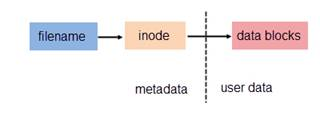
\includegraphics[scale = 1.2]{figure/Link.jpg}	
				\caption{Linux Link Data Access Roud}
				\label{Link}
			\end{figure}
			
			\textbf{查看} \verb|inode| 号可使用命令 \verb|stat 或 ls -i|;
			
			\textbf{查找}\textit{有相同} inode 号的文件 \verb|find / -inum 1114|
			
			\textbf{查看}路径 /home \textit{有相同} inode 的所有硬链接 \verb|find /home -samefile /home/old.file |
			
			\begin{enumerate}
				\item 若一个 \verb|inode |号对应多个文件名,则称这些文件为硬链接。换言之,硬链接就是同一个文件使用了多个别名
				
				\item 软链接与硬链接不同,若文件用户数据块中存放的内容是另一文件的路径名的指向,则该文件就是软连接。软链接就是一个普通文件,只是数据块内容有点特殊。
			\end{enumerate}
			
		
	\section{查看文件}
		\paragraph{cat} 由第一行开始显示文件内容
				\begin{itemize}[itemindent = 1em]
					\item \verb|-b|:列出行号,仅针对非空白行,空白行不标行号。
					\item \verb|-n|:打印出行号,包括空白行
					\item \verb|-v|:列出一些看不出的特殊字符
					\item \verb|-E|:将结尾的断行字符\verb|$|显示出来
					\item \verb|-T|:将\verb|tab |键以\verb|^I|的形式显示出来
					\item \verb|-A|:\verb|-vET| 可以列出特殊字符,而不是以空白代替
				\end{itemize}
		\paragraph{tac} 由最后一行开始显示文件内容, 反向\verb|cat| 输出
			
		\paragraph{nl} 显示的时候,顺道输出行号
		\paragraph{more} 一页一页的显示文件内容
			\begin{itemize}[itemindent = 1em]
				\item \verb|空格 Or f  ->| 翻页
				\item \verb|回车  ->| 换行
				\item \verb|q  ->| 退出
			\end{itemize}
		\paragraph{less} 与\verb|more|类似,但是比\verb|more|更好的是,它\textbf{可以往前翻页}、\textbf{可以查找}
			\begin{itemize}[itemindent = 1em]
				\item \verb|pageUp ->| 向上翻页
				\item \verb|Up  Down ->| 上下换行
				\item \verb|/key ->| 查找, \verb|n 向下查找|
			\end{itemize}
		\paragraph{head} 只看头几行,\verb|head -n 5 ls-text.txt|, 不指定多少行时,默认显式10行。
				
				\verb|-n|:后面接数字,代表显示几行的意思
		\paragraph{tail} 只看尾部几行,\verb|tail -n 5 ls-text.txt|
				\begin{itemize}
					\item \verb|-f| 当文件增长时,输出后续添加的数据
					\item \verb|-s| 与-f合用,表示在每次反复的间隔休眠S秒
				\end{itemize}
			
				为了查看不断更新的日志文件,可以使用的指令\verb|tail -f|
		\paragraph{od} 以二进制的方式读取文件内容
			
		\paragraph{touch} 修改文件时间 或 创建新文件
			
			\subparagraph{文件时间概念}
				\begin{itemize}[itemindent = 1em]
					\item \verb|modification Time(mtime)|:\textbf{当该文件的“内容数据”变更时,就会更新这个时间}!内容数据指的是\textbf{文件的内容},而不是文件的属性或权限喔!
					\item \verb|status Time(ctime)|:\textbf{当该文件的“状态 (status)”改变时,就会更新这个时间},举例来说,像是\textbf{权限与属性}被更改了,都会更新这个时间啊。
					\item \verb|access Time(atime)|:当“该文件的内容被取用”时,就会更新这个读取时间 (access)。举例来说,我们使用 \verb|cat| 去读取 \verb|/etc/man_db.conf |, 就会更新该文件的 \verb|atime| 了。
				\end{itemize}
				
			\subparagraph{touch 选项}
				\begin{itemize}[itemindent = 1em]
					\item \verb|-a|: 修改文件访问时间atime
					\item \verb|-c|: 修改文件的时间ctime
					\item \verb|-m|: 修改文件的mtime
				\end{itemize}
				
	\section{'命令'解释帮助命令}
		\paragraph{man} 查看帮助,\verb|man  级别  命令|,级别含义如下
			\begin{itemize}
				\item \verb|1 |可执行程序或shell 命令【默认】
				\item \verb|2 |系统调用(内核提供的函数)
				\item \verb|3 |库调用(程序库中的函数)
				\item \verb|4 |特殊文件(通常位于/dev)
				\item \verb|5 |配置文件或规范(/etc/passwd)
				\item \verb|6 |游戏
				\item \verb|7 |其他
			\end{itemize}
		\paragraph{type} 说明如何解释命令名:\verb|type  command|
		
		\paragraph{which} 说明会执行在哪块的可执行程序: \verb|which ls| --> /bin/ls
		
		\paragraph{whereis} 说明会可执行程序、配置文件的位置: \verb|which ls| --> /bin/ls
		
		\paragraph{whatis} 显示命令的简要描述:\verb|whatis ls|
		
		\paragraph{man} 显示程序的手册页:\verb|man command|,查看配置文件时切记不要使用绝对路径,当有多个级别的命令时,可以使用-f 指定级别。
		
			
			优先查找命令的帮助、其次是配置文件
			
			当同时存在命令与配置文件时,使用man 时,查看命令添加1\verb|->man 1 passwd|,如果是配置文件则使用5\verb|man 5 passwd|
			
		\paragraph{--help} 显示程序的使用信息:\verb|command --help|
		
		\paragraph{help} 获得\verb|Shell|\textbf{内置命令}(找不到路径的命令)的帮助信息
		
			\verb|->help umask|
			
			\verb|->help if|
		
		\paragraph{apropos} 显示适合的命令:\verb|apropos keyWords|
		
		\paragraph{info} 显示程序的info 条目:\verb|info command|
		\paragraph{alias} 使用别名创建自己的命令:\verb|alias name='command[s]'|
		\paragraph{参考}\url{http://man.linuxde.net}
		
	\section{重定向}这个功能可以把命令行的输入重定向为从文件中获取内容,也可以把命令行的输出结果重定向到文件中。 使用重定向符‘>’,后接文件名,就可以把标准输出重定向到另一个文件中,而不是显示在屏幕上。
	
		当使用重定向符'\verb|>|' 来重定向标准输出时,目的文件通常会从文件开头部分重新改写。如果需要删除一个文件内容(或者创建一个新的空文件),可以采用这样的方式。\verb|> fileName|
		
		如果不需要从文件的首位置开始覆盖文件,而是从文件的\textbf{尾部开始添加内容},我们可以使用重定向符‘\verb|>>|’来实现。
		
		可以使用重定向符\verb|&>| 来把标准输出和标准错误都重定向到同一文件中。
		
		\paragraph{cat}除了查看文件,还可以将不同的文件合并到一个文件里,如 \verb|cat movie*.mpeg >| movie movie.mpeg
		
		\paragraph{管道}命令从标准输入得到数据,并将数据处理后发送到标准输出。使用管道操作符可以把一个命令的输出 传送到另一个命令的标准输入中。 ‘|’	
		\paragraph{sort}按照顺序 排列输入表
		\paragraph{uniq}可以接受来自于标准输入或者一个单个文件名 对应的 已经排好序的数据列表,默认情况下,该命令删除列表中的所有重复行,因此在管道中常与sort 结合使用--> \verb|ls /bin /usr/bin | sort | uniq | less|
		\paragraph{wc}用来显示文件包含的-行数,字数,字节数\verb|-l, -w, -m, -c|。
		\paragraph{tee}从stdin 读取数据,并同时输出到stdout 和 文件
		\paragraph{/dev/null 文件}/dev/null 是一个特殊的文件,写入到它的内容都会被丢弃;如果尝试从该文件读取内容,那么什么也读不到。但是 /dev/null 文件非常有用,将命令的输出重定向到它,会起到"\textbf{禁止输出}"的效果。
	\section{shell扩展}
		\paragraph{echo}把文本参数内容打印到标准输出 :\verb|echo * |--> 打印当前工作目录的所有文件名
		\paragraph{波浪线扩展}如果没有指定用户名,则扩展为当前用户的主目录: \verb|echo ~ --> /home/me   |  \verb|echo ~foo --> /home/foo|
		\paragraph{算术扩展}调用方式:\verb|echo $(( expression ))|
		\paragraph{花括号扩展}\verb|echo F-{A,B,C}-B| --> F-A-B F-B-B F-C-B; \verb|echo n{1..4}| --> n1 n2 n3; 	\verb|echo n{z..a}| --> nz ny nx . na;
		\paragraph{命令  替换}可以把一个命令的输出作为一个扩展模式使用:\verb|echo $(ls)| -->Desktop Documnet Music Pictures.. ,即在需要命令参数处调用\verb|‘$(Command)’|
		\paragraph{双引号扩展}如果把文本放到双引号里,那么所有特殊字符都将失去特殊含义除算数扩展和命令替换
		\paragraph{单引号扩展}如果把文本放到单引号里,那么所有特殊字符都将失去特殊含义,没有除
		
	\section{用户管理}
		\subsection{配置}
			\paragraph{用户信息文件/etc/passwd}可以通过\verb|man 5 passwd|查看。
			
				每行代表一个用户\verb|-> 用户名: 密码标志: UID(用户id): GID(用户初始组): 用户说明: 家目录|
				\verb|: 登录之后的shell|。
			
				\subparagraph{UID}\verb|->|用户标识
					\begin{itemize}
						\item \verb|0| 超级用户
						\item \verb|1~499| 系统用户(伪用户\verb|-> 系统运行时用到的|)
						\item \verb|500~65535| 普通用户
					\end{itemize}
					
					即想把一个普通用户转化成超级用户,\textbf{修改}passwd 配置文件的\textbf{UID段}为0即可。
				
				
			\paragraph{影子文件/etc/shadow}
				每行一个用户\verb|-> 用户名:加密密码:密码最后一次修改日期:两次密码修改间隔|
				 \verb|:密码生效时间:提醒时间:宽限时间|
				 
			\paragraph{组信息文件/etc/group、组密码/etc/gshadow}
			
			
		\subsection{命令}
			\paragraph{useradd} 添加新用户 \verb|: useradd 用户名|	
			
				\begin{itemize}[itemindent = 1em]
					\item \verb|-u ->UID:| 指定用户的UID号
					\item \verb|-d ->家目录:|指定用户的家目录
					\item \verb|-c ->用户说明:|指定用户的说明
					\item \verb|-G ->附加组名:|指定用户的附加组
					\item \verb|-s ->shell:|指定用户的登陆Shell
				\end{itemize}
			
					
				\subparagraph{用户默认值文件}\verb|~|
				
					\verb|/etc/default/useradd ->|
					
					\begin{itemize}[itemindent = 1em]
						\item \verb|GROUP = 100| :用户默认组
						\item \verb|HOME = /home|:用户家目录
						\item \verb|INACTIVE = -1|:密码过期宽限天数
						\item \verb|EXPIRE=|:密码失效天数
						\item \verb|SHELL=/bin/bash|:默认shell
						\item \verb|SKEL=/etc/skel|:模版目录
						\item \verb|CREATE_MAIL_SPOOL=yes|:是否创建目录
					\end{itemize}	
					
					\verb|/etc/login.defs ->|
					
					\begin{itemize}[itemindent = 1em]
						\item \verb|PASS_MAX_DAYS 9999|:密码有效期
						\item \verb|PASS_MIN_DAYS 0|:密码修改时间间隔
						\item \verb|PASS_MIN_LEN 5|:密码最小5位
						\item \verb|PASS_WARN_AGE 7|:密码到其警告
						\item \verb|UID_MIN 500|:最小和最大UID范围
						\item \verb|GID_MAX 60000|
						\item \verb|ENCRYPT_METHOD SHA512|:加密模式 
					\end{itemize}
				\subparagraph{间接影响文件}
					\verb|->|
					
					\begin{lstlisting}
	#useradd sc
	#grep sc /etc/passwd
	#grep sc /etc/shadow
	#grep sc /etc/group
	#grep sc /etc/gshadow
	#ll -d /home/sc/
	#ll /var/spool/mail/sc
	#ll /etc/skel
					\end{lstlisting}
													
			\paragraph{passwd} 更改密码 \verb|-> passwd 用户名|
			
				\verb|root| 可以更改任何人的密码
				
				\verb|普通用户| 只能更改自己的密码
			
				\begin{itemize}[itemindent = 1em]
					\item \verb|-S :|查询用户密码的密码状态。仅root用户可用
					\item \verb|-l :|暂时锁定用户。仅root 用户可用
					\item \verb|-u :|解锁用户。仅root 用户可用
					\item \verb|--stdin :|可以通过管道符输出的数据作为用户的密码。\verb@echo '123'|passwd --stdin user1@
				\end{itemize}
				
			\paragraph{usermod} 修改用户信息,选项同useradd
				\begin{itemize}[itemindent = 1em]
					\item \verb|-c :|修改用户帐号的备注文字
					\item \verb|-d :|修改用户登入时的目录
					\item \verb|-e :|修改帐号的有效期限
					\item \verb|-f :|修改在密码过期后多少天关闭该帐号
					\item \verb|-g :|修改用户所属的群组
					\item \verb|-G :|修改用户所属的附加群组
					\item \verb|-l :|修改用户帐号名称
					\item \verb|-u :|修改用户uid
				\end{itemize}
				
			\paragraph{chage} 修改用户密码状态
				\begin{itemize}[itemindent = 1em]
					\item \verb|-l :|列出用户的详细密码状态
					\item \verb|-d :|修改密码最后一次更改日期(shadow 3字段)
					\item \verb|-m :|两次密码修改间隔(4字段)
					\item \verb|-M :|密码有效期(5字段)
					\item \verb|-W :|密码过期前警告天数(6字段)
					\item \verb|-I :|密码过后宽限天数(7字段)
					\item \verb|-E :|帐号失效时间(8字段)
				\end{itemize}
			
				要求用户初次登录就修改密码:\verb|chage -d 0 user2|
			
			\paragraph{id} 查看用户UID和GID
			
			\paragraph{userdel} 删除用户
				
				\verb|-r :|删除用户的同时删除用户家目录\verb|-> userdel -r User3|,一般都需要加-r选项。
				
			\paragraph{su} 切换用户
				\begin{itemize}
					\item \verb|- :|选项只使用‘-’代表用户的环境变量一起切换
					\item \verb|-c :|仅执行一次命令,而不切换用户身份。
				\end{itemize}
				
				默认情况下\verb|su user1| 切换只是部分切换,而对环境变量不进行改变,可以使用\verb|env |查看。
				
				而‘-c’ 命令经常如下使用:\verb|su - root -c "useradd user3"|,使用root 身份执行一次root 命令但不切换用户。
				
			\paragraph{groupadd} 添加用户组\verb|groupadd 选项 组名|
				
				\verb|-g GID:| 添加指定ID组
			
			\paragraph{groupmod} 修改用户组
				\begin{itemize}[itemindent = 1em]
					\item \verb|-g GID:|修改组ID
					\item \verb|-n 新组名:|修改组名
				\end{itemize}
				
				把组名group1 修改为 test1:\verb|groupmod -n test1 group1|
			
			\paragraph{groupdel} 删除用户组
				\begin{itemize}[itemindent = 1em]
					\item 用户的主组为删除组 不能删除
					\item 其他用户附加组为删除组 不影响删除
				\end{itemize}
				
				
			\paragraph{gpasswd} 把用户加入组或从组中删除。\verb|gpasswd 选项 组名|
				\begin{itemize}[itemindent = 1em]
					\item \verb|-a 用户名:|把用户添加到组
					\item \verb|-d 用户名:|把用户从组中删除
				\end{itemize}	
				
				
			
			\paragraph{who} 查看登陆用户信息
				
				\verb|显式内容-> 用户名 登录终端(tty 本地终端,pts 远程终端)  登陆时间  IP地址|
			
			\paragraph{whoami} 显式当前登陆用户信息
				
			\paragraph{w} 获取更多的登陆用户信息
			
				\verb|显式内容line1-> uptime, 登陆用户个数, load average|
			
				\verb|显式内容line2-> 用户名  登陆终端  IP地址  登入时间 空闲时间   累计占用时间|
					\verb|当前操作占用时间   具体操作|
	\section{权限-基础}
		\subsection{基础}
		\begin{figure}[h]
			\centering
			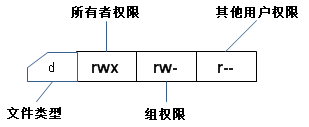
\includegraphics[scale = 1]{figure/fileDescription.png}
			\caption{ls -l 文件权限}
		\end{figure}
		
		\begin{lstlisting}
	Type Owner Group Others
	[-    rwx   rwx   ---]
	[-    111   111   000]
	[-    421   421   000]
	[-     7     7     0 ]
		\end{lstlisting}
		
		\begin{table}[H]
			\centering
			\caption{权限说明}
			\begin{tabular}{m{1cm}|m{1cm}|m{6cm}|m{6cm}}
				\toprule[1.5pt]
				权限	   	  & 含义  & 对文件 &  对目录 \\
				\hline
				\verb|r |	& 读   & 可以查看文件内容\verb|->cat等|& 可以列出目录中的内容\verb|->ls|\\
				\verb|w	|	& 写   & 可以修改文件内容\verb|->vim|& 可以在目录中创建、删除文件\verb|->touch/mkdir/rmdir/rm|\\
				\verb|x	|	& 执行 & 可以执行文件\verb|->script| & 可以进入目录\verb|->cd|\\
				\bottomrule[1.5pt]
			\end{tabular}
		\end{table}	
		
		因此在目录中,有\verb|x执行|权限肯定有\verb|r读|权限
		
	\subsection{命令}
		 \paragraph{chmod}更改文件的模式\verb|-> chmod 权限  文件|
		 
			 chmod 命令符号表示如下:
				\begin{table}[H]
					\centering
					\caption{chmod 作用对象表示法}
					\begin{tabular}{l|m{14cm}}
						\hline
						符号 	   	   & 含义\\
						\hline
						\verb|u |		& user 缩写,表示文件或者目录的所有者\\
						\verb|g	|		& 文件所属群组\\
						\verb|o	|		& others 的缩写,表示其他用户\\
						\verb|a	|		& all 的缩写,是u g o 三者的组合\\
						\verb|+ |		& 添加权利\\
						\verb|-	|		& 删除权利\\
						\verb|=	|		& 赋予权利\\
						\hline
					\end{tabular}
				\end{table}	
			
			如下示例:	
			\begin{lstlisting}[frame=L,xleftmargin=.1\textwidth]
	$chmod u+x test.txt
	--> 给test.txt 的user 添加可执行的权限
			\end{lstlisting}
			
			各种权限可以使用数字来表示,设置权限时可以直接使用数字进行设置:
			
			\verb|chmod Owner+Group+Others file--> chmod 771 file|	 
		 \paragraph{umask}设置文件的默认权限,该值是需要减去的权限. 将给出的掩码与原文件的权限进行\textbf{异或运算},即\textbf{如果掩码为1,那么将该位置的权限擦除}
			 \begin{lstlisting}[frame=L,xleftmargin=.1\textwidth]
	$umask 0002
	--> 设置默认权限 0 000 000 010 :即如果其他用户拥有写权限的话,将擦除该权限
			 \end{lstlisting}
			 
			 如果umask 为022,所以user的权限并没有被拿掉什么权限,但是group 和 others 的权限都被拿掉了2,也就是写(w)权限。
			 \begin{lstlisting}[frame=L,xleftmargin=.1\textwidth]
	$umask 022
	 --> 创建文件时:(-rw-rw-rw-) - (-----w--w-) ==> -rw-r--r--
	 --> 创建目录时:(drwxrwxrwx) - (d----w--w-) ==> drwxr-xr-x
			 \end{lstlisting}
		 \paragraph{chown}只有\verb|root| 用户才可以使用该命令,更改文件所有者, 所有者必须是已经存\textbf{在系统中的帐号},\textit{也就是}在\verb|/etc/passwd |这个文件中有纪录的使用者名称才能改变。
		 \paragraph{chgrp}更改文件所属群组,不过,请记得,要被改变的群组名称必须要在\verb|/etc/group|文件内存在才行,否则就会显示错误!
		 \paragraph{passwd}更改用户密码
	\section{权限-ACL}
		直接针对具体用户 添加具体权限
		
		\paragraph{查看ACL命令} \verb|getfacl 选项 文件名|
		
		\paragraph{设定ACL命令} \verb|setfacl 选项 文件名|
		
			\subparagraph{给特定用户添加对文件(or 目录)特殊权限}\verb|setfacl -m u:用户名:权限 文件或目录|
				\begin{lstlisting}
	// 示例,给用户李四 添加对目录 的读和进入权限
	# useradd zhangsan
	# useradd lisi
	# useradd wangwu
	# groupadd tgroup
	# mkdir /project
	# chown root:tgroup /project
	# chmod 770 /project/
	# setfacl -m u:lisi:rx /project
				\end{lstlisting}
	
			\subparagraph{给特定组添加对文件特殊权限}\verb|setfacl -m g:组名:权限 文件或目录|
		
		\paragraph{ack 最大有效权限}与mask 相与得到的权限,使得给个别用户的权限不会太过。
		
		 \paragraph{chattr} 改变文件属性
			 	\begin{itemize}
			 		\item \verb|+ :|在原有参数设定基础上,追加参数。
			 		\item \verb|- :|在原有参数设定基础上,移除参数。
			 		\item \verb|i :|禁止用户修改,删除,改名
			 		\item \verb|a :|只能向文件中添加数据,而不能删除,多用于服务器日志文件安全,只有root才能设定这个属性。
			 	\end{itemize}
			 	
		 \paragraph{lsattr} 查看文件属性	
	\section{权限-特殊}	 
		 \paragraph{Set UID}\verb|- ..s ... ...|
		 	 \begin{itemize}
		 	 	\item 只有\textbf{可执行文件}\underline{才能设定}\textbf{SUID权限}
		 	 	\item 命令执行者\hspace{.5cm}要对该程序\hspace{.5cm} 拥有执行权限(x)
		 	 	\item 命令执行者\hspace{.5cm} 在执行改程序文件时\hspace{.5cm}获得程序文件属主身份,\verb@A->binary== binaryOwner->binary@
		 	 	\item SetUID 权限\textbf{只在程序执行过程中有效},即\textit{身份改变只在程序执行过程中}有效
		 	 \end{itemize}
		 	
			 普通用户 执行 特定用户的命令时, 短暂时间内 转化为 特定用户,从而拥有一些只有特定用户拥有的权限,从而使用一些特定用户可以的动作。
			 
			 只针对可执行权限x. \verb|x->s|,即只有文件的owner位的权限如下形式才可以完成此操作。
			 
			 \verb|-rws r-x r-x|
			 
			 \textbf{添加该权限}:\verb|chmod u=rwxs file| 或 \verb|chmod u+s file| 或 \verb|chmod 4755 文件名|
			 
			 其中数字4 表示针对用户添加SUID,后面的权限755 意思不变,如果是组的话就是2,是其他用户的话就是1。
			 
		 \paragraph{Set GID}\verb|- ... ..s ...|
		 	 \begin{itemize}
		 	 	\item 只有\textbf{可执行文件或目录}\underline{才能设定}\textbf{SGID权限}
		 	 	\item 命令执行者\hspace{.5cm}要对该程序\hspace{.5cm} 拥有执行权限(x)
		 	 	\item 命令执行者\hspace{.5cm} 在执行改程序文件时\hspace{.5cm} 组身份升级为程序文件的属组,即原A组的a用户执行B组的程序,在执行期间身份自动提升为B组身份
		 	 	\item SetGID 权限\textbf{只在程序执行过程中有效},即\textit{身份改变只在程序执行过程中}有效
 			\end{itemize}
 			
 			\subparagraph{设置SGID} \verb|chmod g+s 文件名| 或 \verb|chmod 2755 文件名|
		 \paragraph{Sticky BIT}\verb|- ... ... ..s|
		 	\begin{itemize}
		 		\item 粘着位 只能\textbf{对目录生效}
		 		\item 普通用户对该目录拥有w 和 x权限,即可以进入并写入。
		 		\item 如果没有粘着位,因为普通用户拥有w权限,那么可以删除其他用户创建的文件。
		 		
		 		而如果赋予粘着位,除了root 可以删除所有文件,普通用户就算拥有w权限,也只能删除自己建立的文件,并且不能删除其他用户建立的文件。
		 	\end{itemize}
		 
		 	\subparagraph{设置粘着位}\verb|chmod o+t 目录名| 或 \verb|chmod 1755 目录名|
		 	
		 \paragraph{UID EUID}
			 \url{http://keren.blog.51cto.com/720558/144908}
			 
		 \paragraph{sudo 权限}
		 	\begin{itemize}
		 		\item root 把本来只能超级用户执行的命令赋予普通用户执行
		 		\item sudo 操作对象是系统命令
		 	\end{itemize}
		 	
		 	首先需要管理员在 \verb|/etc/sudoers| 文件中利用\verb|visudo 命令|完成 对用户可以执行的命令赋予权限。
		 		\begin{lstlisting}
	root ALL=(ALL) ALL
	// 用户名 被赋予管理的地址=(可以使用的身份)  可执行的命令-绝对路径
	sc  ALL=/sbin/shutdown -r now
	sc  192.168.0.156=/usr/bin/vim
	// 不再输密码验证
	sc  localhost=NOPASSWD: /usr/bin/vim
	
	%root ALL=(ALL) ALL
	// 组名  被赋予管理的地址=(可使用的身份)  可执行命令的绝对路径
		 		\end{lstlisting}
		 	
		 	
		 	
		 

	\section{环境/etc}
		\subsection{基本概念}
			login \textbf{shell}[需要输入用户名和密码的] 启动时会读取一个或多个启动文件以配置系统环境:
				\begin{itemize}[itemindent = 1em]
					\item \verb|/etc/profile| 适用于所有用户的全局配置脚本
					\item \verb|~/.bash_profile| 用户个人启动文件,可扩展或重写
					\item \verb|~/.profile|
				\end{itemize}
				
			non-login \textbf{shell} 则会读取以下文件
				\begin{itemize}[itemindent = 1em]
					\item \verb|/etc/bashrc| 适用于所有用户的全局配置脚本
					\item \verb|~/.bashrc| 用户个人启动文件,可扩展或重写
				\end{itemize}
		
		\subsection{相关命令}
		\subparagraph{printenv}打印部分或全部的环境信息
			\begin{table}[H]
				\centering
				\caption{一些必要的环境变量}
				\begin{tabular}{l|m{14cm}}
					\hline
					符号 	   	   & 含义\\
					\hline
					\verb|DISPLAY|		&  运行图形界面环境时界面的名称\\
					\verb|EDITOR|		&  用于文本编辑的程序名称\\
					\verb|SHELL|		&  本机shell 名称\\
					\verb|HOME|		&  本机主目录的路径名\\
					\verb|PWD|		&  当前工作目录\\
					\verb|USER|		&  用户名\\
					\verb|PATH|		&  以冒号分割的一个目录列表,\textbf{当用户输入一个可执行程序的名称时,会查找该目录列表}\\
					\hline
				\end{tabular}
			\end{table}	
			
			\verb|PATH 变量| 通常时由启动文件 \verb|/etc/profile| 中的一段代码设定,但并不如此,取决于系统的发行版本
			\begin{lstlisting}
// 这段代码将$HOME/bin  添加到PATH值的尾部
	PATH = $PATH:$HOME/bin
			\end{lstlisting}
			
			还有一个常见的命令 \verb|export|, 该命令会告诉shell, 将shell的子进程使用\verb|PATH|变量的内容
			\begin{lstlisting}
	export PATH
			\end{lstlisting}
			
			修改环境变量时应当把修改放入以下文件
			\begin{itemize}[itemindent = 1em]
				\item \verb|.bash_profile 或者 其他等效文件(如 Ubuntu中的 .profile)|
			\end{itemize}
			
			其他的改变则应录入\verb|.bashrc|,如
			\begin{lstlisting}
//  .bashrc 文件增加如下代码
	umask 0002
	export HISTSIZE = 1000
	alias ll = 'ls -l --color=auto'
			\end{lstlisting}
			
			但是只要启动shell时才会读取\verb|.bashrc|, 所以对\verb|.bashrc| 做出的修改只有在关闭shell终端回话并重启的时候才会生效。当然我们也可以使用以下命令强制命令bash 重新读取\verb|.bashrc| 文件
			
			\begin{lstlisting}
	$source .bashrc
			\end{lstlisting}
		\subparagraph{set}设置shell 选项
		\subparagraph{export}将环境导出到随后要运行的程序中
		
	\section{VI 编辑器}
		\subsection{基本模式}
			\begin{itemize}
				\item 普通模式
				\item 插入模式
				\item 可视模式
				\item 选择模式
				\item 命令行模式
				\item ex模式
			\end{itemize}
			\begin{figure}[h]
				\centering
				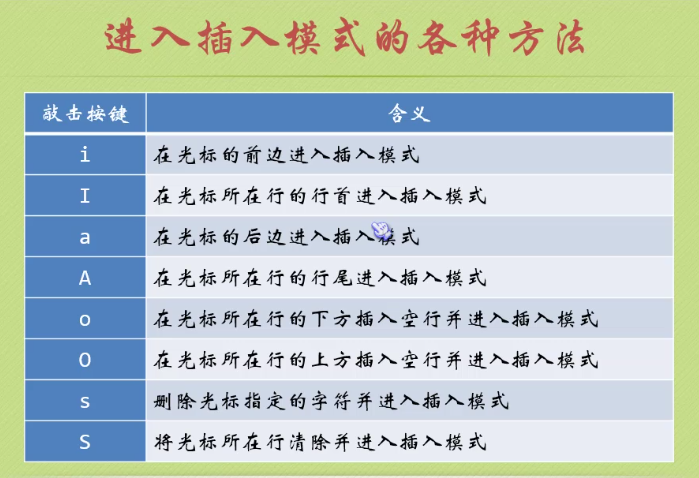
\includegraphics[scale = 0.5]{figure/viInsert.png}
				\caption{vi插入示例}
			\end{figure}

		\subsection{模式转换}
			模式如下,所有在\textbf{使用命令的时候一般需要按Esc按键返回到命令模式下才可以.}.而并非在插入模式与ex转义方式下。
			通过输入vi的插入命令(i)、附加命令(a)、打开命令(o)、替换命令(s)、修改命令(c)或取代命令(r)可以从命令方式进入输入方式。
			\begin{figure}[h]
				\centering
				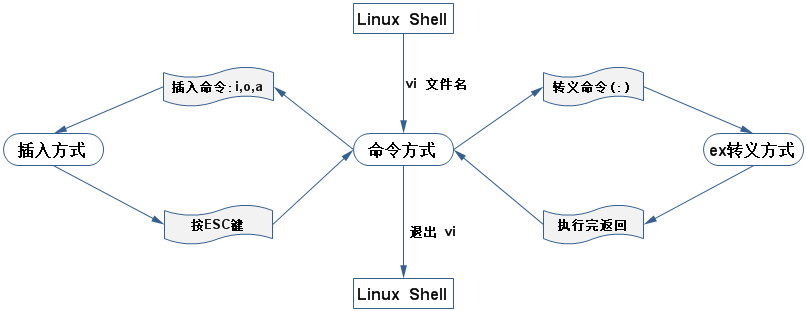
\includegraphics[scale = 0.5]{figure/vi.png}
				\caption{vi模式转换示例}
			\end{figure}
		
		\subsection{常用命令}
			\url{http://blog.csdn.net/weixin_40910753/article/details/79077074}
			
			$$\verb|数字奥义(单,范围)| + \verb|命令| + \verb|正则光标|$$
			
			\paragraph{选中一块区域并缩进缩出}\verb|->|
				\subparagraph{可视模式}
					按\verb|ESC| 进入正常模式
					\begin{enumerate}[itemindent = 1em]
						\item 按\verb|v|进入视觉模式
						\item 按\verb|shift|,移动上下键选择文本
						\item \verb|>| 缩进,\verb|<| 缩出
					\end{enumerate}
					
				\subparagraph{正常模式}
					按\verb|ESC| 进入正常模式
					
					\verb|数字的奥义| + \verb@>>|<<@
					
			\paragraph{移动光标}\verb|->|
			
				按\verb|ESC| 进入正常模式
				\subparagraph{数字0} 移动光标至本行开头,\verb|Home| 也有此功能
				\subparagraph{\$} 移动光标至本行末尾,\verb|End| 也有此功能
				\subparagraph{gg} 移动光标到文件第一行
				\subparagraph{G} 移动光标到文件最后一行
				\subparagraph{b} 移动光标到该单词的第一个字母
				\subparagraph{e} 移动光标到该单词的最后一个字母
				\subparagraph{w} 移动光标到下一个单词的起始处
				\subparagraph{num+G} 移动光标到第 \verb|num| 行
				
			\paragraph{删除操作}\verb|->|
			
				按\verb|ESC| 进入正常模式
				\subparagraph{x} 删除当前字符
				\subparagraph{d0}删除当前光标到行开头字符
				\subparagraph{d\$}删除当前光标到结尾字符
				\subparagraph{dW} 删除整个单词
				\subparagraph{dd} 删除当前行
				\subparagraph{d+G} 删除当前行到文件末尾
				\subparagraph{num+dd} 删除与本行在内的往后 \verb|num| 行
				
					\verb|数字 + motion = | 重复多个motion
				\subparagraph{d+num+G} 删除当前行到第\verb|num|行
				\subparagraph{:n1,n2d} 删除n1 到n2 行
				
			\paragraph{撤销恢复}\verb|->|	
				\subparagraph{u} undo  操作
				\subparagraph{ctrl+r} redo 操作
			
			\paragraph{复制粘贴}\verb|->|

				按\verb|ESC| 进入正常模式
				\subparagraph{y0}复制当前光标到行开头字符
				\subparagraph{y\$}复制当前光标到结尾字符
				\subparagraph{yW} 复制整个单词
				\subparagraph{yy} 复制当前行
				\subparagraph{num+yy} 复制连同当前行往后的num行
				\subparagraph{y+num+G} 复制当前行到文件第num行
				\subparagraph{y+G} 复制当前行到文件末尾
				\subparagraph{p} 粘贴复制文本到当前光标\textbf{前}
				\subparagraph{P} 粘贴复制文本到当前光标\textbf{后}
				\subparagraph{J} 合并后一行至当前行
				\url{https://stackoverflow.com/questions/2770739/vim-error-e492-not-an-editor-command-dd}
				
			\paragraph{查找}\verb|->|
			
				按\verb|ESC| 进入正常模式
				\subparagraph{'/keyword'} 在当前文本 向后查找 \verb|keyword|
				\subparagraph{'?keyword'} 在当前文本 向前查找 \verb|keyword|
				\subparagraph{n} 寻找下一个 
				\subparagraph{N} 寻找上一个 
				\subparagraph{\%} 快速\textbf{匹配括号}
				
			\paragraph{全局搜索和替换}\verb|->|
			
				\verb|esc : 进入ex 模式|
				\begin{table}[H]
					\centering
					\caption{ex 搜索替换使用规范}
					\begin{tabular}{l|m{13cm}}
						\hline
						符号 	   	   & 含义\\
						\hline
						\verb|:|	&  分号用于启动一条ex 命令\\
						\verb|% |	 &  确定作用范围,\verb|%|代表从文件的第一行到最后一行,\verb|1,5| 代表第一行到第5行,\verb|2,$| 代表从第二行到最后一行. 如果不指定范围的话,只会在当前行生效\\
						\verb|s |	 &  指定了具体的操作- 本次操作为替换操作(搜索和替换)\\
						\verb|s/find/replace|		&  搜索find关机字,并将其替换为replace\\
						\verb|r |	 &  取代光标所在处字符\\
						\verb|R |	 &  从光标所在处开始替换字符,按Esc 结束\\
						\verb|g |	 &  替换正行\\
						\verb|c |	 &  确认是否替换\\
						\hline
					\end{tabular}
				\end{table}	
				
				\verb|:%s/find/replace/g| 全文将find 替换为 replace
				
				\verb|:1,4s/find/replace/gc| 将第一行到第4行的find 全部替换为 replace,并询问确认意见
				
				\url{http://blog.sina.com.cn/s/blog_736f1c59010136ry.html}
				
			\paragraph{查找删除注释}\verb|->|
				\subparagraph{'s/old/new/ '}用old替换new,替换当前行的第一个匹配
				\subparagraph{'s/old/new/g '}用old替换new,替换当前行的所有匹配
				\subparagraph{'\%s/old/new/'}用old替换new,替换所有行的第一个匹配
				\subparagraph{'\%s/old/new/g'}用old替换new,替换整个文件的所有匹配
				\subparagraph{',5 s/\^ /\#/g'} 注释当前行到第5行
				\subparagraph{',+5 s/\^ /\#/g'} 注释当前行与之后的5行
				\subparagraph{'3,5 s/\^ \#//g'} 解除3-5行的注释	
			
			\paragraph{查看目录下有什么文件}\verb|->|
			
				\verb|:! command|
				
				\verb|:! ls /| 列出根目录文件		
					
			\paragraph{文件保存}\verb|->|
			
				\verb|esc : 进入ex 模式|
				\subparagraph{:w} 保存修改
				\subparagraph{:wq} 保存修改并退出
				\subparagraph{:q!} 不保存修改退出
				\subparagraph{:wq!} 强行保存并退出(文件所有者和root 可以使用)
				
			\paragraph{局部另存为}\verb|->|
					\begin{itemize}
						\item \verb|esc  v|进程可视模式
						\item \verb|shift |选中文本
						\item \verb|:w newFileName| 将选中的另存为newFileName
					\end{itemize}			
				
				\subparagraph{文件覆盖}
					\verb|:w! oldFile| 将oldfile 用现有内容覆盖
						
						
				\subparagraph{文件合并}
					\verb|:r file| 将file文件的内容 合并到当前文件 光标的下方。
					
					\textit{技巧}:结合重定向技巧将bash 命令执行结果写入文件中如\verb|:r !date|
			\paragraph{编辑多文本}\verb|->|
				\url{https://www.cnblogs.com/end/archive/2012/06/12/2546757.html}
				\subparagraph{vi file1 file2 }
					\begin{itemize}[itemindent = 2em]
						\item \verb|-o| 垂直并排
						\item \verb|-O| 水平并排
						\item \verb|ctrl + w + w| 切换到下一个文件
						\item \verb|ctrl + w + 方向键| 切换到相对位置的文件
						\item \verb|a| 作用于所有,在ex模式下使用\verb|:wa :qa|
					\end{itemize}
				
				\subparagraph{在不同窗口中打开多个文件}	
					如果\textbf{已经打开}一个了一个文件,
					
					\begin{itemize}[itemindent = 2em]
						\item \verb|esc :|进入命令模式
						\item \verb|:sp newFile|水平分割继续打开第二个文件
						\item \verb|:vsp newFile|纵向分割打开第二个文件
					\end{itemize}
				
					或者用 \verb|vi -o file1 file2 file3....|用\textbf{分割屏幕窗口方式同时打开多个文件}。
					
				\subparagraph{分屏操作}
					\begin{itemize}[itemindent = 2em]
						\item \verb|ctrl+w s|   对当前文档内容分屏显示
						\item \verb|ctrl+w q|   关闭所处分屏
						\item \verb|ctrl+w o |  仅显示当前分屏内容
					\end{itemize}
				
				\subparagraph{n 与 N} 切换下一个文件
				\subparagraph{:buffers} 显示当前打开的文件们
				\subparagraph{:buffer num} 切换到文件num
				
				\subparagraph{:e newfile}[*常用] 载入更多的文件,然后使用\verb|ctrl + ^|在文件之间切换
				
					\begin{itemize}[itemindent = 2em]
						\item \verb|:ls|  展示全部的打开文档
						
						\item \verb|:xn|  切换到向下的第x个文档
						
						\item \verb|n ctrl+6 |切换到第n个buffer
						
						\item \verb|ctrl+6  或 :e#|   回到前一个编辑文件
					\end{itemize}
				
				
				
				
				\subparagraph{:tabe}
				\url{http://blog.csdn.net/achang21/article/details/44562253}
				\subparagraph{文件间复制} 跟普通复制粘贴一样,只是需要切换目标文件先
				
				\subparagraph{插入整个文件} \verb|:r insertFile| 将insertFile 的内容插入到光标位置之前 	
		
		\subsection{配置}
			\url{https://segmentfault.com/a/1190000011466454}
			
			\subsubsection{.vimrc}
				\verb|.vimrc| 是 \verb|Vim| 的配置文件,需要我们自己创建
				\begin{lstlisting}
	cd Home               // 进入 Home 目录
	touch .vimrc          // 配置文件
	
	# 安装插件管理工具 vim-plug
	# Unix
	# Vim
	curl -fLo ~/.vim/autoload/plug.vim --create-dirs \
	https://raw.githubusercontent.com/junegunn/vim-plug/master/plug.vim
	# Neovim
	curl -fLo ~/.local/share/nvim/site/autoload/plug.vim --create-dirs \
	https://raw.githubusercontent.com/junegunn/vim-plug/master/plug.vim
				\end{lstlisting}
			
			\subsubsection{基本配置}
				\begin{itemize}
					\item 文件编码 \verb|set encoding=utf-8|
					\item 显示行号 \verb|set number|
					\item 显示光标当前位置 \verb|set ruler|
					\item 设置缩进 
					    \begin{lstlisting}
	set cindent	
	set tabstop=2
	set shiftwidth=2
					    \end{lstlisting}
				    
					\item  突出显示当前行 \verb|set cursorline|
				\end{itemize}
				
			\subsubsection{插件配置}
				\subparagraph{树形目录}Plug 'scrooloose/nerdtree', 使用\verb|shit+r |动态刷新目录。
				\subparagraph{代码补全}Plug 'Valloric/YouCompleteMe'
				\subparagraph{git显示}Plug 'airblade/vim-gitgutter'
							
		\subsection{常用插件}
			\subsection{vundle 插件管理器}
				\url{http://blog.csdn.net/myloveqingmu/article/details/52518563}
			
			
			\url{http://blog.csdn.net/mergerly/article/details/51671890}
			
			\url{http://blog.csdn.net/jack__cj/article/details/52671312}
			\subsubsection{ctags}
				安装:\url{http://blog.csdn.net/u013445530/article/details/46726109}
				
				tags下载:\url{https://wiki.geany.org/tags/start}
				\begin{enumerate}
					\item 安装软件:\verb|sudo apt-get install ctags|
					\item 下载补全资源:\verb|.h|
					\item 生成tags文件:ctag 生成 \verb|tags|文件
					\item 使用:\verb|ctrl+p| 与 \verb|ctrl+n| 使用
				\end{enumerate}
			
			\subsection{Gtags}
				
			\subsection{NERDTree}
			
			\subsection{Tagbar}
			
			\subsubsection{YouCompleteMe}
				
	\section{存储介质挂载}
		\paragraph{挂载点的意义}
			每个 \verb|filesystem| 都有独立的 \verb|inode、 block 、superblock| 等信息,\textbf{这个文件系统}\textit{要能够}\textbf{链接到目录树}\underline{才能}\textbf{被我们使用}。 \textbf{将文件系统与目录树结合的动作我们称为“ 挂载 ”}。 
			
			重点是: \textbf{挂载点一定是目录},\textit{该目录为进入该文件系统的入口}。 因此并不是你有任何文件系统都能使用,必须要“挂载”到目录树的某个目录后,才能够使用该文件系统的。
			
		\paragraph{挂载}
			\begin{itemize}
				\item windows \verb|->| 硬件设备映射为一个盘符
				\item linux \verb| ->| 将硬件设备挂载成(映射到)一个目录
			\end{itemize}

			linux 的每个挂载了分区的目录 就相当于 windows系统中的盘符,比如/home/ftp 和 /oracle目录我们就可以把她看做一个盘符和一个分区关联
			
			\url{http://blog.csdn.net/gongweijiao/article/details/8425629}
		\paragraph{mount}查询系统中已经挂载的设备
		
			\verb|mount [-t 文件系统] [-o 特殊选项]  设备文件名  挂载目录|
			
			\begin{itemize}
				\item \verb|-a| 依据配置文件\verb|/etc/fstab|的内容,开机自动挂载
				\item \verb|-t| 文件系统类型可以有 ext3, ext4, fat16, fat32等
				\item \verb|-o| 可以指定挂载的额外选项
			\end{itemize}
		
			\verb|-> 挂载U盘|:此盘在windows下格式化为fat32文件系统
				\begin{enumerate}
					\item 挂u盘之前,运行命令\verb|cat /proc/partitions|,\textbf{看看现在系统中有哪些分区}。插上u盘以后,再次运行上述命令,看看多出来什么分区(通常是sda1或者 sdb1)
					
					\item 输入 \verb|fdisk -l /dev/sda| 查看输出结果,\textbf{决定以什么文件系统挂载}。
					\begin{lstlisting}[frame=L,xleftmargin=.1\textwidth]
	#fdisk -l /dev/sda 
	 Disk /dev/sda: 131 MB, 131104768 bytes      
	 3 heads, 32 sectors/track, 2667 cylinders      
	 Units = cylinders of 96 * 512 = 49152 bytes 
	 Device Boot      Start         End      Blocks   Id System     
	/dev/sdb1   *           1        2668      128016    6 FAT16
					\end{lstlisting}
					
					\item 根据文件系统类型挂载,如\verb|mount -t msdos /dev/sdb1 /mnt/usb|
					
					可以使用\verb|cat /proc/filesystems |查看当前系统支持的文件系统格式
						\begin{itemize}
							\item 如果是\verb|fat16|格式,就用命令:  \verb|mount -t msdos /dev/sdb1 /mnt/usb| 
							\item 如果是\verb|fat32|格式,就用命令: 	\verb|mount -t vfat /dev/sdb1 /mnt/usb -o iocharset=utf8 |
							\item 如果是\verb|ext2| 格式,就用命令:  \verb|mount -t ext2 /dev/sda1 /mnt/usb|
							\item 如果是\verb|NTFS| 格式,就用命令:  \verb|mount -t ntfs /dev/sda1 /mnt/usb|
						\end{itemize}
				\end{enumerate}
				
				挂载实例:\url{https://wenku.baidu.com/view/ef8aa226dd36a32d73758139.html}
				
			\paragraph{umount} 如果需要挂载其他盘,则需要卸载\verb|umount 设备名|
			
	\section{网络}
			\paragraph{write} 给指定\textbf{在线用户}发信息,以\verb|Ctrl+D|保存结束
			
				\verb|write  用户名  消息   Ctrl-D结束输入|
			
			\paragraph{wall} 给所用在线用户发送消息,广播
			
				\verb|wall   消息|
				
			\paragraph{ping} \textbf{向网络主机发送特殊数据包}(\verb|ICMP ECHO_REQUEST|). 多数网络设备收到该数据包后会做出回应,通过此法可判断网络链接(两者间)是否正常. \verb|ping  baidu.com|
			
				指定ping 的\textbf{次数}:\verb|ping -c 3 baidu.com| ping 3次百度。
			
			\paragraph{ifconfig} 查看和设置网卡信息
			
				\subparagraph{查看} \verb|ifconfig|
				
				\subparagraph{设置} \verb|ifconfig eth0 192.168.1.12|
				
				\verb|service network restart|
				
			\paragraph{mail} 查看发送电子邮件
				
				发送:\verb|mail 用户  消息  Ctrl-D结束|
				
				接受:\verb|mail|
					\begin{itemize}[itemindent = 1em]
						\item 查看,输入序列号即可
						\item 删除,d 序列号
					\end{itemize}
			
			\paragraph{last} 列出目前与过去登入系统的用户信息\verb|->last|
				
			\paragraph{traceroute} \textbf{跟踪网络数据包的传输路径},会显示文件通过网络从本地系统到指定主机过程中所有停靠点的列表。 \verb|traceroute  slashdot.org|
			
			\paragraph{netstat} 检查网络设置以及相关统计数据,\verb|-ie|可以检查系统的网络接口信息,\verb|-r| 可以显示内核的网络路由表
				\url{http://www.cnblogs.com/ggjucheng/archive/2012/01/08/2316661.html}
				
				\begin{table}[H]
					\centering
					\begin{tabular}{l|m{12cm}}
						\hline
						\verb|netstat |   	   & \verb|options| \\
						\hline
						\verb| |   	   & \verb|-a |(\verb|all|)显示所有选项,默认不显示\verb|LISTEN|相关 \\
						\verb| |   	   & \verb|-t |(\verb|tcp|)仅显示\verb|tcp|相关选项\\
						\verb| |   	   & \verb|-u |(\verb|udp|)仅显示\verb|udp|相关选项 \\
						\verb| |   	   & \verb|-n |拒绝显示别名,能显示数字的全部转化成数字 \\
						\verb|netstat |   	   & \verb|-l |仅列出有在 \verb|Listen| (监听) 的服務状态\\
						\verb| |   	   & \verb|-p |显示建立相关链接的程序名 \\
						\verb| |   	   & \verb|-r |显示路由信息,路由表 \\
						\verb| |   	   & \verb|-e |显示扩展信息,例如\verb|uid|等\\
						\verb| |   	   & \verb|-s |按各个协议进行统计 \\
						\verb| |   	   & \verb|-c |每隔一个固定时间,执行该\verb|netstat|命令\\
						\hline
					\end{tabular}
				\end{table}	
					
				\verb|LISTEN和LISTENING|的状态只有用\verb|-a|或者\verb|-l|才能看到
				
				\begin{itemize}[itemindent = 1em]
					\item 列出所有 \verb|tcp| 端口: \verb|netstat -at|
					\item 列出所有 \verb|udp| 端口: \verb|netstat -au|
					\item 只列出所有处于监听状态 \verb|tcp| 端口: \verb|netstat -lt|
					\item 显示\verb|tcp|和进程名称 \verb|netstat -pt|
				\end{itemize}
				
			\paragraph{ftp:lftp:sftp} \verb|File Transfer Protocol|,ftp 服务器 就是那些包含供 网络上传、下载文件的机器
				\begin{table}[H]
					\centering
					\caption{FTP 使用说明}
					\begin{tabular}{l|m{13cm}}
						\hline
						命令 	   	   & 含义\\
						\hline
						\verb|ftp server|	&  建立 FTP 连接,在命令上中先输入\verb|ftp|然后空格跟上 \verb|FTP 服务器的域名 'domain.com'| 或者 \verb|IP 地址|\\
						\verb|anonymous|	 &  使用用户名密码登录,绝大多数的 \textbf{FTP 服务器是使用密码保护的},因此这些 FTP 服务器会询问\verb|'username'|和\verb|'password'|.	如果你连接到被称作匿名 FTP 服务器,可以尝试\verb|anonymous|作为用户名以及使用空密码:\verb|Name: anonymous, Password:|\\
						\verb|目录操作|	 &  FTP 命令可以列出、移动和创建文件夹,如同我们在本地使用我们的电脑一样。\verb|ls|可以打印目录列表,\verb|cd|可以改变目录,\verb|mkdir|可以创建文件夹\\
						\verb|使用 FTP 下载文件|		&  在下载一个文件之前,我们首先需要使用\verb|lcd|命令\textbf{设定本地接受目录位置}。
						\verb|lcd /home/user/yourdirectoryname| 如果你不指定下载目录,文件将会下载到你登录 FTP 时候的工作目录。现在,我们可以使用命令 \verb|get| \textbf{来下载文件},比如:\verb|get file|\textbf{文件会保存在}使用\verb|lcd|命令设置的目录位置\\
						\verb|使用 FTP 上传文件|	 &  使用 \verb|put|命令上传文件:\verb|put file|\\
						\verb|关闭 FTP 链接| &  \verb|quit exit bye|3 个命令都可以\\
						\hline
					\end{tabular}
				\end{table}	
				
			\paragraph{wget} 非交互式网络下载工具 \verb|wget http://www.linuxde.net/testfile.zip|
			
			\paragraph{*远程操作 ssh} 安全登录远程计算机:SSH 解决了与远程主机进行安全通信的两个基本问题:1、该协议可以验证远程主机的身份是否真实;2、该协议将本机与远程主机之间的通信内容全部加密
				
				SSH协议 包括2部分:1、运行在远程主机上的SSH服务端,用来监听端口\textbf{22} 上可能过来的连接请求;2、是本地系统上的SSH客户端,用来与远程服务器进行通信
				
			关于SSH 的相关命令有 \verb|scp|,\verb|sftp|,分别表示远程拷贝 和 更简单高效快速的ftp
			
			例如:执行\verb|ssh happycast.net|命令,然后输入密码,接着就可以直接访问该服务器..但是每次连接都得输入密码我们可以使用以下步骤进行简化:
				\begin{lstlisting}
	$ssh-keygen
	$cd ~/.ssh
	$ls
	id_rsa  id_rsa.pub
	
	// 然后我们把公钥id_rsa.pub 上传至服务器/home/Usr1/.ssh/authorized_keys即可
	$ssh-copy-id 服务器名(Usrl@happycasts.net)
				\end{lstlisting}
			
			\paragraph{*数据传输 rsync}见归档备份
			
			\paragraph{nc}\verb|netcat|所做的就是在两台电脑之间建立链接并返回两个数据流,在这之后所能做的事就看你的想像力了。你能建立一个服务器,传输文件,与朋友聊天,传输流媒体或者用它作为其它协议的独立客户端。
				
				\url{http://blog.csdn.net/zhangxiao93/article/details/52705642}
				\begin{itemize}[itemindent = 1em]
					\item 端口扫描
					\item ChatServer
					\item 文件传输
				\end{itemize}
				
			\paragraph{pv}是 \verb|Pipe Viewer| 的简称,意思是通过管道显示数据处理进度的信息。这些信息包括已经耗费的时间,完成的百分比(通过进度条显示),\textit{当前的速度,全部传输的数据,以及估计剩余的时间}。
			
				\url{http://www.jb51.net/LINUXjishu/409870.html}
				
			\paragraph{tcpdump}
				
				\url{http://www.cnblogs.com/ggjucheng/archive/2012/01/14/2322659.html}
				\begin{itemize}[itemindent = 1em]
					\item 监视指定主机的数据包
						\begin{itemize}
							\item 打印所有\textbf{进入或离开}\verb|sundown|的数据包:
							
								\verb|tcpdump host sundown| 或 \verb|tcpdump host 210.27.48.1 |
							\item 打印helios \textbf{与} hot \textbf{或者与} ace 之间通信的数据包
							
								\verb|tcpdump host helios and \( hot or ace \)| 或 
								
							    \verb|tcpdump host 210.27.48.1 and \ (210.27.48.2 or 210.27.48.3 \)| 
							\item  打印ace \textbf{与} 任何不是\verb|helios|主机 通信的IP 数据包
							
								\verb|tcpdump ip host ace and not helios| 或 
								
								\verb|tcpdump ip host 210.27.48.1 and ! 210.27.48.2|
							\item 截获主机\verb|hostname|\textbf{发送的}所有数据
							
								\verb|tcpdump -i eth0 src host hostname|
							\item 监视所有\textbf{送到}主机\verb|hostname|的数据包
							
								\verb|tcpdump -i eth0 dst host hostname|
						\end{itemize}
						
					\item 获取主机\verb|10.2.4.1|在端口23上\textbf{接收或发出}的包:
							\verb|tcpdump tcp port 23 and host 10.2.4.1|
					
					\item  () 得使用转义字符进行,要么不识别
					
						\verb|tcpdump \(src 172.17.14.98 and dst 172.17.15.112\) or \(src 172.17.15.112 and dst 172.17.14.98\)|
				\end{itemize}
				
			\paragraph{iperf}可以测试\verb|TCP和UDP|带宽质量。\verb|iperf|可以报告带宽,延迟抖动和数据包丢失。
			
			\paragraph{ifconfig}
			
			\paragraph{iptables}
			
			\paragraph{vmstate} vmstat命令是最常见的\textbf{Linux/Unix监控工具},可以展现\textbf{给定时间间隔}的\textbf{服务器的状态值},包括服务器的\textbf{CPU使用率,内存使用,虚拟内存交换情况,IO读写情况}
			
			\verb|-> 使用:|
			
			\verb|vmstat [-a] [-n] [-S unit] [delay [ count]]|
			
			\verb|vmstat [-s] [-n] [-S unit]|
			
			\verb|vmstat [-m] [-n] [delay [ count]]|
			
			\verb|vmstat [-d] [-n] [delay [ count]]|
			
			\verb|vmstat [-p disk partition] [-n] [delay [ count]]|
			
			\verb|vmstat [-f]|
			
			
			\begin{table}[H]
				\centering
				\begin{tabular}{l|m{14cm}}
					\hline
					\verb|参数 |   	   & \verb|含义| \\
					\hline
					\verb|delay |      & 刷新时间间隔。如果不指定,只显示一条结果。	\\
					\verb|count |      & 刷新次数。如果不指定刷新次数,但指定了刷新时间间隔,这时刷新次数为无穷。	\\
					\verb|-a |   	   & 开启显示active/inactive memory	\\
					\verb|-f |   	   & 显示此系统启动以来的forks的总数,包括fork、vfork和clone system calls	\\
					\verb|-m |   	   & 显示slabinfo信息	\\
					\verb|-n |   	   & 只显示头信息,不周期性显示.也就是说开启这个参数,只显示头部信息一次。	\\
					\verb|-s |   	   & 显示各种事件计数器表和内存统计信息,这显示不重复	\\
					\verb|-d |   	   & 显示磁盘统计数据	\\
					\verb|-w |   	   & 可以扩大字段长度,当内存较大时,默认长度不够完全展示内存。	\\
					\verb|-p |   	   & 显示磁盘分区数据	\\
					\verb|-S |   	   & 参数S控制输出性能指标的单位,k(1000) K(1024) 或 M(1048576) 默认单位为K(1024 bytes)	\\
					\hline
				\end{tabular}
			\end{table}	
			
		 \url{http://www.cnblogs.com/tommyli/p/3746187.html}
		 
		 \url{http://www.cnblogs.com/ggjucheng/archive/2012/01/05/2312625.html}
		 
	\section{通配符}
		通配符是用于匹配符合条件的\textbf{文件名},通配符是\textbf{完全匹配。}包括\verb|任意个*  一个? 括号中的一个[x]|
		
		\verb|ls、find、cp|这些命令不支持正则表达式,所以只能使用通配符来进行匹配。
		
		
	\section{正则表达式}
		正则表达式用来在\textbf{文件中}匹配符合条件的\textbf{字符串},正则是\textbf{包含匹配}。
		
		\verb|grep、awk、sed| 等命令支持正则表达式
		
		$$\verb|正则表达式|=
			\begin{cases}
				\verb|字符类|\\
				\verb|数量限定类|\\
				\verb|位置限定类|
			\end{cases}$$	
		
		\url{http://www.cnblogs.com/hanxiaoyu/p/5759477.html}

		\subsection{字符类}
			\begin{table}[H]
				\centering
				\begin{tabular}{l|m{7cm}|m{8cm}}
					\hline
					\verb|字符 |   	   & \verb|含义| & \verb|例子|\\
					\hline
					\verb|. |   	   & 匹配任意一个字符 & \verb|abc. |可以匹配 \verb|abcd、 abc9| 		\\
					\verb|[]|   	   & 匹配括号中的任意一个字符 & \verb|[abc]d |可以匹配 \verb|ad、 bd、cd|		\\
					\verb|- |   	   & 在\verb|[]|中使用,表示字符范围 &\verb|[0-9 a-f A-F] |可以匹配一位16进制数字	\\
					\verb|^ |   	   & 位于括号内的开头,匹配括号中的字符外的任意一个字符 &\verb|[^xy]  |可以匹配 除\verb|x、y|之外的任一字符		\\
					\verb|[[:xx:]]|	   & 预定义的一些命名字符 & \verb|[[:digit:]] |匹配一个数字    \\
					\hline
				\end{tabular}
			\end{table}	
		
			\verb|[\d]| 等价于 \verb|[0-9]|
			
			\verb|/ |只是在某些语言中作为正则的\textbf{边界符},如sed 在匹配正则时,不仅要指定r, 正则还要以'/'开头
		\subsection{数量限定类}
			\begin{table}[H]
				\centering
				\begin{tabular}{l|m{8cm}|m{7cm}}
					\hline
					\verb|字符 |   	   & \verb|含义| & \verb|例子|\\
					\hline
					\verb|? |   	   & 紧跟在他前面的单元应匹配0次或1次 & \verb|[0-9]?\.[0-9] |匹配 \verb|0.0 2.3  .5|等,特殊字符\verb|.| 需要加转义字符 		\\
					\verb|+ |   	   & 紧跟在他前面的单元应匹配1次或多次 & \verb|[a-zA-Z0-9_-]+ @| \verb|[a-zA-Z0-9_.-]+ \.|\verb|[a-zA-Z0-9_.-]+| 匹配email 地址 \\
					\verb|* |   	   & 紧跟在他前面的单元应匹配0次或多次 & \verb|[0-9]* |匹配至少1位数字	 \\
					\verb|{N}|   	   & 紧跟在他前面的单元应精确匹配N次 & \verb|[1-9][0-9]{2} |匹配100到999的整数	\\
					\verb|{N,}|	  	   & 紧跟在他前面的单元应匹配至少N次 & \verb|[1-9][0-9]{2,} |匹配3位及3位以上的整数   \\
					\verb|{,M}|   	   & 紧跟在他前面的单元应匹配最多M次 & \verb|[0-9]{,1} |最多匹配一次数字	\\
					\verb|{N,M}|	   & 紧跟在他前面的单元应匹配至少N次,最多M次 &  \verb|[0-9]{1,3} |表示0-9数字至少匹配1次,最多匹配3次 \\
					\hline
				\end{tabular}
			\end{table}	
			
		\subsection{位置限定类}
			\begin{table}[H]
					\centering
				\begin{tabular}{l|m{8cm}|m{7cm}}
					\hline
						\verb|字符 |   	   & \verb|含义| & \verb|例子|\\
					\hline
						\verb|^ |   	   & 匹配行首的位置 & 	\verb|^content | 匹配行首为content的行\\
						\verb|$ |   	   & 匹配行末的位置 &  \verb|;$ |匹配行末尾为 \verb|;|的行, \verb|^$ |匹配空行\\
						\verb|\<|   	   & 匹配单词开头的位置 & \verb|\<th |匹配.. this..,但不匹配 tenth等 \\
						\verb|\>|   	   & 匹配单词结尾的位置 & \verb|p\> |匹配leap, 但不匹配 parent\\
						\verb|\b|	  	   & 匹配单词的开头\verb|\bx|或结尾\verb|x\b|的位置 & \verb|\b at|匹配 at,但不匹配 batch\\
						\verb|\B|   	   & 匹配非单词开头\verb|\Bx|或结尾的位置 & \verb|\B at|匹配 battery, 但不匹配 attend、hat\\
					\hline
				\end{tabular}
			\end{table}
		
		\subsection{特殊字符}
			\begin{table}[H]
				\centering
				\begin{tabular}{l|m{8cm}|m{7cm}}
					\hline
					\verb|字符 |   	   & \verb|含义| & \verb|例子|\\
					\hline
					\verb|\ |   	   & 转义字符  & 	\\
					\verb|() |   	   & 将正则表达式的一部分括起来组成一个单元,可以对整个单元使用数量限定符&  \verb|([0-9]{1,3}\.){3}[0-9]{1,3}| 匹配IP地址\\
					|   	   & 链接两个子表达式,表示或的关系 &  \\
					\hline
				\end{tabular}
			\end{table}		
	\section{搜索命令}
		\paragraph{*文件搜索命令 locate} 通过 \verb|[部分]文件名| 查找\textbf{文件} 的具体位置,搜索速度比\verb|find| 快。在后台数据库中按文件名搜索,搜索数据速度更快,但是后台数据库更新一般是1天更新一次,但是可以使用\verb|updatedb|强制更新后台数据库。
		
			但是使用\verb|updatedb |时遵循\verb|/etc/updatedb.conf|配置文件的规则
			\begin{itemize}[itemindent = 1em]
				\item 开启搜索限制 \verb|PRUNE_BIND_MOUTS = "yes"|
				\item 搜索时,不搜索的文件系统 \verb|PRUNEFS = |
				\item 搜索时,不搜索的文件类型 \verb|PRUNENAMES = |
				\item 搜索时,不搜索的路径 \verb|PRUNEPATHS =|,默认包含\verb|\tmp| 
			\end{itemize}
			
			当配置文件开启搜索规则时,update命令执行后,locate会在搜索时遵照updatedb.conf规则进行剔除搜索。
			
			\textbf{选项}\verb|->|
			\begin{itemize}[itemindent = 1em]
				\item \verb|-i|:忽略大小写
				\item \verb|-c|:不输出文件名,仅计算找到的文件数量
				\item \verb|-l|:仅输出结果的几行,例如输出5行则是 \verb|-l 5|
			\end{itemize}
		
		\paragraph{*文件搜索命令 find}	在文件系统目录框架中查找文件(\textbf{完全匹配})
		
			\hspace{1cm} \verb|find path -option [-print -delete -ls -quit] [[-exec -ok] command{}[; +]]| 
	
			\begin{table}[H]
				\centering
				\begin{tabular}{l|m{7cm}|m{8cm}}
					\hline
					\verb|find |   	   & \verb|options| & \verb|含义|\\
					\hline
					\verb| |   	   & \verb|-name   filename |& 	查找名为\verb|filename|的文件	\\
					\verb| |   	   & \verb|-perm | & 			按执行权限来查找	\\
					\verb| |   	   & \verb|-user   username | & 按文件属主来查找					\\
					\verb| |   	   & \verb|-group  groupname | &按组来查找 					\\
					\verb| |   	   & \verb|-mmin  -n +n | & 	按文件内容修改时间来查找文件(分钟)	-n 多少分钟以内		\\
					\verb|find |   & \verb|-mtime  -n +n | & 	按文件更改时间来查找文件,\verb|-n|指\verb|n|天以内,\verb|+n|指\verb|n|天以前				\\
					\verb| |   	   & \verb|-atime  -n +n | &	按文件访问时间来查				\\
					\verb| |   	   & \verb|-ctime  -n +n | & 	按文件属性修改时间来查找文件,\verb|-n|指\verb|n|天以内,\verb|+n|指\verb|n|天以前				\\
					\verb| |   	   & \verb|-newer  f1 !f2| & 	查更改时间比\verb|f1|新但比\verb|f2|旧的文件				\\
					\verb| |   	   & \verb|-type   b/d/c/p/l/f |&查是块设备b、目录d、字符设备c、管道p、符号链接l、普通文件f 		\\
					\verb| |   	   & \verb|-size   n[c] | & 	查长度为\verb|n|块[或\verb|n|字节]的文件,\verb|-小于size的,+大于size的|, \verb|find /etc -size +20k -a -size -50k|	\\
					\verb| |	   & \verb|-inum   fileNum|			&   查找文件节点号为fileNum 的文件\\
					\verb| |   	   & \verb|-mount | & 			查文件时不跨越文件系统\verb|mount|点		\\
					\verb| |	   & \verb|-and -or| & \verb|-and|条件与 \verb|-or|条件或\\
					\hline
				\end{tabular}
			\end{table}	
			
			\begin{itemize}
				\item  \verb|-print| 将查找到的文件输出到标准输出
				\item  \verb|-exec   command   {} \;|      —–将查到的文件执行command操作,\verb|{}|为查找的结果,也是新命令的参数。
				\item  \verb|-ok |和\verb|-exec|的作用相同,只不过以一种更为安全的模式来执行该参数所给出的shell命令,在执行每一个命令之前,都会给出提示,让用户来确定是否执行。
			\end{itemize}
			
			\textbf{通配符}\verb|*任意内容  ?任意一个字符  []任意一个括号内的字符|
		
			\hspace{1cm} \url{http://www.cnblogs.com/wanqieddy/archive/2011/06/09/2076785.html}
			
		\paragraph{*字符串搜索命令 grep}\textit{把匹配的}\textbf{行}\verb| |打印出来。使用正则的都是\textbf{包含匹配},grep 也不例外
		
			\verb|-> grep "正则"  文本|
			
			\verb@-> |grep 选项  字符串Or正则@
			\begin{table}[H]
				\centering
				\begin{tabular}{l|m{7cm}|m{8cm}}
					\hline
					\verb|grep |   	   & \verb|options| & \verb|regex pattern|\\
					\hline
					\verb| |   	   & \verb|-c |只输出匹配行的计数 & \verb|\   |忽略正则表达式中特殊字符的原有含义\\
					\verb| |   	   & \verb|-i |不区分大 小写(只适用于单字符) & \verb|^   |匹配正则表达式的开始行\\
					\verb| |       & \verb|-e |并列使用多个 \verb|-e|参数可以实现\textbf{或}条件					& \verb| netstat -an || \verb|grep -e EST -e WAIT|\\
					\verb| |   	   & \verb|-h |查询多文件时不显示文件名 & \verb|$   |匹配正则表达式的结束行\\
					\verb| |   	   & \verb|-l |查询多文件时只输出包含匹配字符的文件名 & \verb|\<  |从匹配正则表达 式的行开始\\
					\verb| |   	   & \verb|-n |显示匹配行及 行号& \verb|\>  |到匹配正则表达式的行结束\\
					\verb| |   	   & \verb|-s |不显示不存在或无匹配文本的错误信息 & \verb|[ ] |单个字符,如[A]即A符合要求\\
					\verb| |   	   & \verb|-v |不显示包含匹配文本的所有行 & \verb|*  | 有字符,长度可以为0\\
					\verb| |   	   & \verb|-r |递归的对目录下的所有文件(包括子目录)进行 grep & \\
					\verb| |   	   & & \verb|[ - ]|范围,如[A-Z],即A、B、C一直到Z都符合要求\\
					\hline
				\end{tabular}
			\end{table}		
			
			\verb@cat /etc/passwd | grep /bin/bash | grep -v root@:在passwd 文件中截取默认登录shell 为/bin/bash即普通用户,然后并包包含root用户.
		\paragraph{命令搜索命令 whereis 与 which}
			\verb|which|指令会在环境变量\verb|$PATH|设置的目录里查找符合条件的文件。
			
			\verb|whereis|指令会在特定目录中查找符合条件 的文件。这些文件的属性应属于原始代码,二进制文件,或是帮助文件。
			
		\paragraph{xargs} 从标准输入中建立、执行命令行,一般结合 管道 | 在结果中使用。
		
			\hspace{1cm} \verb|find ~ -type f -name 'foo*' -print | | \verb|xargs ls -l|

		\paragraph{stat} 显示文件或文件系统的状态
	
	\section{文本相关}
		\dirtree{%		
					.1 字符截取.
					.2 截取行.
					.3 grep.
					.3 sed.
					.2 截取列.
					.3 cut.
					.3 awk.
				}
				
		\paragraph{sed}sed是一个很好的文件处理工具,本身是一个管道命令,主要是\textbf{以行为单位进行处理},可以将数据行进行替换、删除、新增、选取等特定工作
			
			\verb|sed [options] 'command' 输入文本|
			
			\subparagraph{选项}
				\begin{itemize}[itemindent = 1em]
					\item \verb|-n|∶使用安静(silent)模式。在一般 sed 的用法中,所有来自 STDIN的资料一般都会被列出到萤幕上。但如果加上 -n 参数后,则只有经过sed 特殊处理的那一行(或者动作)才会被列出来。
					
					\item \verb|-e|∶直接在指令列模式上进行 sed 的动作编辑;
					    
					\item \verb|-f|∶直接将 sed 的动作写在一个档案内, -f filename 则可以执行 filename 内的sed 动作;
					
					\item \verb|-r|∶sed 的动作支援的是延伸型正规表示法的语法。(预设是基础正规表示法语法)
					   
					\item \verb|-i|∶直接修改读取的档案内容,而不是由萤幕输出。
				\end{itemize}
			\subparagraph{命令}
				\begin{itemize}[itemindent = 1em]
					 \item \verb|a |  ∶\textbf{新增}, a 的后面可以接字串,而这些字串会在新的一行出现(目前的下一行)
					 \item \verb|c |  ∶\textbf{取代}, c 的后面可以接字串,这些字串可以取代 n1,n2 之间的行!
					 \item \verb|d |  ∶\textbf{删除},因为是删除啊,所以 d 后面通常不接任何咚咚;
					 \item \verb|i |  ∶\textbf{插入}, i 的后面可以接字串,而这些字串会在新的一行出现(目前的上一行);
					 \item \verb|p |  ∶\textbf{列印},亦即将某个选择的资料印出。通常 p 会与参数 sed -n 一起运作
					 \item \verb|s |  ∶\textbf{取代},可以直接进行取代的工作哩!通常这个 s 的动作可以搭配正规表示法!例如 \verb|1,20s/old/new/g|
				\end{itemize}
		
		\url{http://www.cnblogs.com/dong008259/archive/2011/12/07/2279897.html}
		
		\paragraph{awk}	
			\verb|awk '条件1{动作1} 条件2{动作2}...' 文件名|, 先读入一行,然后逐行执行操作。
			
			\subparagraph{条件 Pattern}一般使用关系表达式作为条件
				\begin{itemize}[itemindent = 1em]
					\item \verb|x > 10|
					\item \verb|x >= 10|
					\item \verb|x <= 10|
				\end{itemize}
		
			\subparagraph{动作 Action}
				\begin{itemize}[itemindent = 1em]
					\item 格式化输出
					\item 流程控制语句
				\end{itemize}
		
			\subparagraph{例子}
				\begin{itemize}
					\item \verb|awk ' {printf $2 "\t" $6 "\n"}'   student.txt|  :patten 省略,表示对每行都执行,显式文件中的第2列和第6列。
					\item \verb@df -h|awk '{print $1 "\t" $3}' @: 截取df 输出的第1列和第三列, 与cut 不同的是,awk 无须指定分割符,并且需要注意的是,print 会自动分行,但是格式控制与printf 相同。
					\item 
				\end{itemize}			
			\subparagraph{BEGIN} 在其他所有命令逐行执行前,执行一次 BEGIN后的动作
			
				\verb|awk 'BEGIN{print "Test awk BEGIN"} {print $2 "\t" $5}'  student.txt|
				
				这条命令首先执行BEGIN 后的 print Anction, 然后逐行读取数据执行之后的条件与动作。
		
			\subparagraph{FS内置变量} 指定分隔符
			
				\verb|awk '{FS=":"}{print $1"\t"$3}'  /etc/passwd|
				
				这条命令意思是指定分割符为:,但是在读入第一行后,再执行后面Action 时,指定分隔符已经来不及了,所以这种情况第一行时不会正确使用分割符分割的,而是从第2行开始的,为了解决这个问题,可以利用前面提到的BEGIN 解决。
				
				\verb|awk 'BEGIN{FS=":"}{xx}'  xx|
			
			\subparagraph{END} 在所有命令执行完后,执行一次 END后的动作
				
				\verb|awk '{print $1"\t"$3}  END{print"The End"}'  student.txt|	
				
			
			\subparagraph{关系运算}
				\verb@cat fileName.txt | grep -v Name | awk '$6 >= 87 {print $2}'@
		\paragraph{cat} 连接文件并打印到标准输出
			\begin{itemize}
				\item -A, --show-all 等价于 -vET
				\item -b, --number-nonblank 对非空输出行编号
				\item -e 等价于 -vE
				\item -E, --show-ends 在每行结束处显示\verb| $|
				\item -n, --number 对输出的所有行编号
				\item -s, --squeeze-blank 不输出多行空行
				\item -t 与 -vT 等价
				\item -T, --show-tabs 将跳 字符显示为 \verb|^I|
			\end{itemize}
		
		\paragraph{sort} 对\textbf{文本行}排序..
			\begin{itemize}
				\item \verb|-r |默认升序,使用-r 选项使用降序
				\item \verb|-t |设定分隔符,如存在按列分割,然后按照第几列排序时,需要指定分割符
				\item \verb|-k |按照第几列排序
				\item \verb|-u |去除重复行
				\item \verb|-n |按照数值排序,解决按照字符串排序的尴尬(1 > 10 > 2),加了-n 后(1,2,10)
			\end{itemize}
		
		\paragraph{wc} 对\textbf{文本}进行统计 \verb|wc 选项 文件|
		
			\begin{itemize}
				\item \verb|-1 |只统计行数
				\item \verb|-w |只统计单词数
				\item \verb|-m |只统计字符数
			\end{itemize}
			
		\paragraph{uniq} 报告并省略重复行
		
		\paragraph{cut}\verb|cut 选项 文件名|,有局限,仅支持制表符、和常用分隔符(,:。-),不支持空格。
			\begin{itemize}
				\item \verb|-f列号 |提取第几列
				\item \verb|-d分隔符 |按照指定分隔符分割列
			\end{itemize}
			
			\verb|cut -f 2 student.txt| 提取文件第2列
			
			\verb|cut -f 2,3 student.txt| 提取文件第2列和第三列
			
			\verb|cut -d ":" -f 1,3 /etc/passwd| 截取第一列和第三列,并且分隔符号为:
		
		\paragraph{paste} 合并文件文本行
		
		\paragraph{join} 基于某个共享字段来联合两个文件的 文本行
		
		\paragraph{comm} 逐行比较 两个已经排序好 的文件
		
		\paragraph{diff} 逐行比较文件
		
		\paragraph{patch} 对原文件打补丁
		
		\paragraph{tr} 转换或删除 字符
		
		\paragraph{aspelx} 交互式拼写检查器
		
		
	\section{归档备份}
		\subsection{压缩与解压缩}常见格式有\verb|.zip  .gz  .bz2  .tar.gz  .tar.bz2|
			
				\begin{itemize}
					\item  \verb|.zip|
						\begin{itemize}
							\item \textbf{压缩} 
								\begin{enumerate}
									\item \verb|zip 压缩文件名  源文件|:压缩文件
									\item \verb|zip -r 压缩文件名 源目录|:压缩目录
								\end{enumerate}
							\item \textbf{解压缩} \verb|unzip 压缩文件|
						\end{itemize}
					
					\item  \verb|.gz|
						\begin{itemize}
							\item \textbf{压缩}
								\begin{enumerate}
									\item \verb|gzip 源文件|:压缩为\verb|.gz|格式的压缩文件,源文件会消失
									\item \verb|gzip -c 源文件 > 压缩文件|:压缩为\verb|.gz|格式,源文件保留
									\item \verb|gzip -r 目录|:压缩目录下所有子文件,但是不能压缩目录
								\end{enumerate}
							\item \textbf{解压缩}
								\begin{enumerate}
									\item \verb|gzip -d 压缩文件|:解压缩文件
									\item \verb|gunzip 压缩文件|:解压缩文件
									\item \verb|解压目录加-r 即可|
								\end{enumerate}
						\end{itemize}
						
					\item  \verb|.bz2|
						\begin{itemize}
							\item \textbf{压缩},不能压缩目录
								\begin{enumerate}
									\item \verb|bzip2 源文件|:压缩为\verb|.bz2|格式,不保留源文件
									\item \verb|bzip2 -k 源文件|:压缩后保留原文件
								\end{enumerate}
							\item \textbf{解压缩},加关键字-k 保留压缩文件
								\begin{enumerate}
									\item \verb|bzip2 -d 压缩文件|
									\item \verb|bunzip2 压缩文件|
								\end{enumerate}
						\end{itemize}
					
					\item \textbf{打包}\verb| tar -cvf 打包文件名 源文件|
						\begin{enumerate}
							\item \verb|-c| 打包
							\item \verb|-v| 显示过程
							\item \verb|-f| 指定打包后的文件名
						\end{enumerate}
						
						\verb|tar -cvf long.tar long|
						
						将文件直接打包后压缩为\verb|.tar.gz|格式,-z前缀
						\begin{enumerate}
							\item \verb|-z| \textbf{压缩}为\verb|.tar.gz|:\verb|tar -zcvf 压缩文件名  原文件|
							\item \verb|-x| \textbf{解压缩}\verb|.tar.gz|:\verb|tar -zxvf 压缩包名|
						\end{enumerate}
						
						将文件直接打包后压缩为\verb|.tar.bz2|格式,-j前缀
						\begin{enumerate}
							\item \verb|-z| \textbf{压缩}为\verb|.tar.bz2|:\verb|tar -jcvf 压缩文件名  原文件|
							\item \verb|-x| \textbf{解压缩}\verb|.tar.bz2|:\verb|tar -jxvf 压缩包名|
							\item \verb|-C| 解压到指定路径下\verb|tar -jxvf test.tat.bz2 -C /tmp/|
						\end{enumerate}
						
				\end{itemize}
		
		\subsection{同步文件和目录}
			\paragraph{rsync}在对rsync服务器配置结束以后,下一步就需要在客户端发出rsync命令来实现将服务器端的文件备份到客户端来,但是也可以同步本地的文件夹等,命令格式如下:
				\begin{lstlisting}
rsync [OPTION]... SRC DEST
rsync [OPTION]... SRC [USER@]HOST:DEST
rsync [OPTION]... [USER@]HOST:SRC DEST
rsync [OPTION]... [USER@]HOST::SRC DEST
rsync [OPTION]... SRC [USER@]HOST::DEST
rsync [OPTION]... rsync://[USER@]HOST[:PORT]/SRC [DEST]
				\end{lstlisting}
				
			对应于以上六种命令格式,rsync有六种不同的工作模式:
				\begin{itemize}
					\item 拷贝本地文件。当\verb|SRC|和\verb|DES|路径信息都不包含有单个冒号”\verb|:|”分隔符时就启动这种工作模式。如:\verb|rsync -a /data /backup|
					\item 使用一个远程shell程序(如rsh、ssh)来实现将本地机器的内容拷贝到远程机器。当\verb|DST|路径地址包含单个冒号”\verb|:|”分隔符时启动该模式。如:\verb|rsync -avz *.c foo:src|
					\item 使用一个远程shell程序(如rsh、ssh)来实现将远程机器的内容拷贝到本地机器。当\verb|SRC|地址路径包含单个冒号”\verb|:|”分隔符时启动该模式。如:\verb|rsync -avz foo:src/bar /data|
					\item 从远程rsync服务器中拷贝文件到本地机。当\verb|SRC|路径信息包含”\verb|::|”分隔符时启动该模式。如:\verb|rsync -av root@172.16.78.192::www /databack|
					\item 从本地机器拷贝文件到远程\verb|rsync|服务器中。当\verb|DST|路径信息包含”::”分隔符时启动该模式。如:\verb|rsync -av /databack root@172.16.78.192::www|
					\item 列远程机的文件列表。这类似于\verb|rsync|传输,不过只要在命令中省略掉本地机信息即可。如:\verb|rsync -v rsync://172.16.78.192/www|
				\end{itemize}
				
			\url{http://www.cnblogs.com/subsir/articles/2565373.html}

		\subsection{备份}
			\paragraph{备份策略}完全备份、\textbf{增量备份}、差异备份(与完全备份相比)
			
			\paragraph{dump}增量备份:\verb|dump 选项 备份之后的文件名  原文件或目录|
				\begin{itemize}
					\item -level :0-9 备份级别,0 表示基本备份, 以后增加level,表示第多少次增量备份, 并且\textbf{目录不支持增量备份}
					\item -f :指定备份之后的文件名
					\item -u :备份成功后,把备份时间记录在\verb|/etc/dumpdates| 文件
					\item -v :显式备份过程中输出的信息
					\item -j :调用bzlib 库压缩备份文件\verb|.bz2|
					\item -W :显式运行被dump 的分区的备份等级及备份时间
				\end{itemize}
				
			\paragraph{restore}\verb|restore [模式选项] [选项]|
				\begin{itemize}
					\item -C :比较备份数据和实际数据的变化 
					\item -i :进入交互模式,手工选择需要恢复的文件
					\item -t :查看模式,用于查看备份文件中拥有哪些数据
					\item -r :还原模式,数据还原
					\item -f :指定备份文件的文件名
				\end{itemize}
	\section{进程管理}
		\paragraph{ps}\textbf{显示当前}所有进程的运行情况,显式格式为\verb|USER  PID  %CPU %MEM  VSZ  TSS TTY ...|,具体表示为
			\begin{itemize}
				\item \verb|USER :|该进程由哪个用户产生的
				\item \verb|PID :|该进程的ID号
				\item \verb|%CPU :|该进程占用CPU资源百分比
				\item \verb|%MEM :|该进程占用物理内存百分比
				\item \verb|VSZ :|该进程占用虚拟内存百分比
				\item \verb|RSS :|该进程占用实际物理内存的大小
				\item \verb|TTY :|该进程在哪个终端中运行的
				\item \verb|STAT :|进程状态。R 运行、S 睡眠、T 停止、s 包含子进程、+ 位于后台
				\item \verb|START :|该进程的启动时间
				\item \verb|TIME :|该进程占用CPU的运算时间,注意不是系统时间
				\item \verb|COMMAND :|产生此进程的命令名
			\end{itemize}
			
			将程序\textit{运行至后台}..\verb|xxCommand &|
			
				\begin{table}[H]
					\centering
					\caption{ps 参数含义}
					\begin{tabular}{l|m{14cm}}
						\hline
						符号 	   	   & 含义\\
						\hline
						\verb|l |		&  长格式输出\\
						\verb|u	|		&  按用户名和启动时间的顺序来显示进程\\
						\verb|j	|		&  用任务格式来显示进程\\
						\verb|f	|		&  用树形格式来显示进程\\
						\verb|a |		&  显示所有用户的所有进程(包括其它用户)如:\verb|ps a| \textit{显示现行终端机下的所有程序}\\
						\verb|x	|		&  显示无控制终端的进程\\
						\verb|r	|		&  显示运行中的进程\\
						\hline
					\end{tabular}
				\end{table}	
				参考:\url{http://www.cnblogs.com/wangkangluo1/archive/2011/09/23/2185938.html}
		
		\paragraph{top} 查看系统健康状态,\textbf{实时动态显示}当前所有任务的资源占用情况
			\begin{itemize}
				\item 系统信息
				\item 进程信息
				\item \verb|CPU|信息
				\item 物理内存信息
				\item 交换区信息
				\item ps 信息
			\end{itemize}
		
		\paragraph{pstree} 进程树,显式进程的父子关系
		
		\paragraph{kill}发送信号给某个进程,\verb|kill 选项 进程号|
			\subparagraph{kill -l} 查看可用的进程\textbf{信号}。常用信号如下:
				\begin{itemize}
					\item \verb|SIGHUP 1:|该信号让进程立即关闭,然后重新读取配置文件之后重启
					\item \verb|SIGINT 2:|程序终止信号,用于终止前台进程。相当于<Ctr-c>
					\item \verb|SIGFPE 8:|算术致命运算错误
					\item \verb|SIGKILL 9:|用于立即结束程序的运行,本信号不能被阻塞、处理。一般用于强制终止进程
					\item \verb|SIGALRM 14:|时钟定时信号,alarm 函数使用该信号
					\item \verb|SIGTERM 15:|正常结束进程信号
					\item \verb|SIGCONT 18:|该信号让暂停的进程恢复执行,本信号不能被阻断
					\item \verb|SIGSTOP 19:|该信号暂停前台进程,相当于<Ctr-z>									
				\end{itemize}
			
			\subparagraph{killall} 杀死指定名字的进程。\verb|killall 选项 进程名:|杀死\textbf{进程名}的所有进程,注意不是\textbf{进程号}
			
			\subparagraph{pkill} -t 按照终端号踢出进程。	
			
		\paragraph{后台执行}
				\verb|Command &|(后台运行命令)
				
				\textbf{特点:}是执行后\textbf{命令行不会一直占用},可以执行其他命令.例如
				\begin{lstlisting}
	$firefox &
	...
	
	$Available..
				\end{lstlisting}
				
			\subparagraph{ctrl+z} 暂停当前运行进程,并放入后台,(后台暂停命令)
			\subparagraph{ctrl+c} 结束当前运行进程
			\subparagraph{jobs}列出所有活动作业的状态信息\verb|工作号 工作状态  工作进程|
			
			\subparagraph{bg}设置在后台中运行作业\verb|bg %工作号|, 如果不想添加工作号,默认执行工作号后面有[+] 的,接下来是[-],如\verb|bg \n|。
			
				注意:在把后台暂停的工作恢复到后台执行的过程中,后台恢复的执行的命令是不能和前台有交互的,否则不能恢复到后台执行。如\verb|top Vi|
			
			\subparagraph{fg}设置在前台中运行作业\verb|fg %工作号|,第二种方式如bg,直接运行\verb|fg|即可。
		
		\paragraph{lsof} 列出进程打开或使用的文件信息
			\begin{itemize}
				\item \verb|-c 字符串:|只列出以字符串开头的进程打开的文件
				\item \verb|-u 用户名:|列出某个用户的进程打开的文件
				\item \verb|-p pid:|列出某个pid进程打开的文件
			\end{itemize}	
			
	\section{服务管理}
		\begin{itemize}
			\item 包安装服务
				\begin{itemize}
					\item 独立的服务
					\item 基于\verb|xinetd|服务		
				\end{itemize}
			\item 源码包服务 
		\end{itemize}	
	
		\paragraph{查询已安装的服务-包安装与源码安装服务}
			查看包安装的服务\verb|chkconfig --list|, 查看服务的自启动状态,\verb|service| 只能管理包安装的服务,不能管理源码安装的服务。主要原因是\textbf{安装位置的区别}。
		
			查看源码服务安装位置,一般是\verb|/usr/local| 下
			
		\paragraph{包安装-独立服务的启动与自启}
			\begin{itemize}
				\item \verb|/etc/init.d/ :|启动脚本位置
				\item \verb|/etc/sysconfig/ :|初始化环境配置文件位置
				\item \verb|/etc/ :|配置文件位置
				\item \verb|/etc/xinetd.conf :|xinetd 配置文件
				\item \verb|/etc/xinetd.d/ :|基于xinetd 服务的启动脚本
				\item \verb|/var/lib/ :|服务产生数据放在这里 
				\item \verb|/var/log/ :|日志
			\end{itemize}
			
			\subparagraph{启动}
				\begin{itemize}[itemindent = 1em]
					\item 标准方式:\verb@/etc/init.d/独立服务名  start|stop|status|restart|@-> 服务绝对路径 + 操作
					\item \verb@service 独立服务名 start|stop|status|restart|@-> 在默认目录中搜索服务名 + 操作
				\end{itemize}
			
			\subparagraph{查询安装服务的状态}
				\verb|service --status -all|
			
			\subparagraph{服务自启动}
				\begin{itemize}[itemindent = 1em]
					\item 命令方式:chkconfig --level 运行级别 服务名 on(off)
					\item 标准方式:修改\verb|/etc/rc.d/rc.local 文件|,输入用户民和密码之前,会执行该文件里保存的命令
					\item 其他:使用\verb|ntsysv 命令|管理自启动
				\end{itemize}
			
		\paragraph{包安装- xinetd服务的启动与自启}几乎不使用了,被淘汰了,现在只有telnet 在使用。
		
		\paragraph{源码安装- 服务的启动与自启}
			\subparagraph{启动}
				\begin{itemize}[itemindent = 1em]
					\item 使用绝对路径
					\item 调用\textbf{启动脚本}来启动。不同的源码包的启动脚本不同,可以查看源码包安装说明,查看启动脚本的方法
				\end{itemize}
				
				\verb@usr/local/apache2/bin/apachetcl   start|stop@
		
			\subparagraph{自启动}
				\begin{itemize}[itemindent = 1em]
					\item 修改\verb|/etc/rc.d/rc.local|,加入脚本启动命令\verb@usr/local/apache2/bin/apachetcl   start@
					\item 创建快捷方式至 service 执行时的搜索目录\verb|/etc/init.d/|,然后执行\verb|service 服务名  start|即可
				\end{itemize}
				
				\verb|让源码包的服务| 可以被\verb|chkconfig 与 ntsysv| 识别,需要在\verb|/etc/init.d/链接文件| 中添加如下内容,并执行\verb|chkconfig --add 服务链接文件|
					\begin{lstlisting}
	#chkconfig: 35 86 76
	#chkconfig: 运行级别  启动顺序 关闭顺序
	#description: source package apache
	#说明,内容随意
					\end{lstlisting}
			
	\section{系统管理}
		\subsection{资源管理}
			\paragraph{缓冲与缓存}缓存(cache)用于加速数据从硬盘\textbf{读取}的。 缓冲(buffer)是用于加速数据\textbf{写入}硬盘的
			
			\paragraph{vmstat}top 精简版-监控系统资源(\verb|memory swap  io  system  cpu|):\verb|vmstat  刷新延时  刷新次数|
			
			\paragraph{dmesg}开机时内核检测信息
	
			\paragraph{free}查看内存使用状态:\verb@free [-b|-k|-m|-g]@
				\begin{itemize}
					\item \verb|-b:|以字节显式
					\item \verb|-k:|以KB显式
					\item \verb|-m:|以MB显式
					\item \verb|-g:|以GB显式
				\end{itemize}
			
			\paragraph{/proc/cpuinfo} 保存cpu 信息,查看cpu 可以通过此文件、也可以通过vmstat, 也可以通过 top。
			
			\paragraph{uptime} 显式系统的启动时间 和 平均负载,也就是top 命令的第一行。w 命令也可以看到这个数据。
			
			\paragraph{uname} 查看系统与内核相关信息
				\begin{itemize}
					\item \verb|-a :|查看系统所有相关信息
					\item \verb|-r :|查看内核版本
					\item \verb|-s :|查看内核名称
				\end{itemize}
				
			\paragraph{file /bin/外部命令} 判断当前系统位数\verb|file /bin/ls  file /bin/find|
			
			\paragraph{lsb\_release -a}查看当前Linux 系统发行版本
		
		\subsection{定时任务}
			\paragraph{crond 服务:crontab}\verb|crontab [选项]|
				\begin{itemize}
					\item \verb|-e:|编辑crontab 定时任务
					\item \verb|-l:|查询crontab 任务
					\item \verb|-r:|删除当前用户所有的crontab 任务
				\end{itemize}
			
				\subparagraph{任务脚本格式}\verb|* * * * * 执行的任务|
					\begin{table}[H]
						\centering
						\caption{crontab参数含义}
						\begin{tabular}{p{3cm}<{\centering}|p{5cm}<{\centering}|p{6cm}<{\centering}}
							\toprule[1.5pt]
							项	   	   & 含义 & 范围\\
							\hline
							\verb|第1个* |&一小时当中的第几分钟  &0-59 \\
							\verb|第2个* |&一天 当中的第几个小时 &0-23 \\
							\verb|第3个* |&一月 当中的第几天  &1-31 \\
							\verb|第4个* |&一年 当中的第几月  &1-12 \\
							\verb|第5个* |&一周 当中的星期几  &0-7(0和7都代表星期日) \\
							\verb|*|& 代表任何时间 &比如第一个*就代表一小时的每一分钟都执行一次的意思\\
							\verb|,|& 代表不联系时间 &比如第一个* 替换为‘0,8,14’ 则表示为每小时的第0,8,14 分钟执行命令\\
							\verb|-|& 代表连续的时间范围 &比如第一个* 替换为0-13,则表示为每小时的第0分钟到第13分钟执行命令\\
							\verb|*/n|& 代表每隔多久执行一次 &比如第一个替换为*/10,则表示为每隔10分钟执行一次命令\\
							\bottomrule[1.5pt]
						\end{tabular}
					\end{table}	
				
				\subparagraph{示例}\verb|->|	
					\begin{itemize}[itemindent =1em]
						\item \verb|45 22 * * * 命令 :|在22点45分执行命令 
						\item \verb|0 17 * * 1 命令 :|每周1 的17点0分执行命令
						\item \verb|0 5 1,15 * * 命令 :|每月1号和15号的5点0分执行命令
						\item \verb|40 4 * * 1-5 命令 :|每周1到每周5,即工作日内每天4点40分执行命令
						\item \verb|*/10 4 * * * 命令 :|每天4点,每隔10分钟执行一次命令
						\item \verb|0 0 1,15 * 1 命令 :|每月1号和15号,每周1的 0点0分都会执行命令。
						\item \verb|0 5 1,10,14 * * /root/sh/autobak.sh :|每月1,10,14号的5点执行脚本autobak.sh
					\end{itemize}
				
			
	\section{日志管理}
		\subsection{常见日志}
			\paragraph{/var/log/cron}记录了系统定时任务相关的日志
			
			\paragraph{/var/log/cups/}记录打印信息的日志
			
			\paragraph{/var/log/dmesg}记录了系统在开机时内核自检的信息。也可以使用dmesg 命令直接查看内核自检信息。
			
			\paragraph{/var/log/btmp}记录错误登陆的日志。这个文件时2进制文件,不能直接使用vi 查看,需要使用lastb 命令查看。
			
			\paragraph{/var/log/lastlog}记录系统中所有用户最后一次的登录时间的日志。也同样是二进制文件,需要使用lastlog 命令查看。
			
		\subsection{rsyslogd 日志服务}
			\paragraph{日志文件格式}
				\begin{itemize}
					\item 事件产生的时间
					\item 发生事件的服务器的主机名
					\item 产生事件的服务名或程序名
					\item 事件的具体信息
				\end{itemize}
			
			\paragraph{日志配置文件}\verb|/etc/rsyslog.conf|
			
				配置格式:\verb|服务名称[连接符号]日志等级    日志记录位置 -> authpriv.*   /var/log/secure|
			
				\subparagraph{常见服务名称}
					\begin{itemize}[itemindent = 1em]
						\item auth: 安全和认证相关信息
						\item authpriv:安全和认证相关信息
						\item cron:系统定时任务cront 和 at 产生的日志
						\item daemon:各个守护进程产生的日志
						\item ftp:ftp守护进程产生的日志
						\item kern:内核产生的日志
					\end{itemize}
					
				\subparagraph{连接符号}
					\begin{itemize}[itemindent = 1em]
						\item \verb|* |代表所有的日志等级
						\item \verb|. |代表只有比后面的级别高的日志都记录下来
						\item \verb|= |代表只记录所需等级的日志
						\item \verb|.! |代表不等于,也就是除了该等级的日志外,其他等级都记录
					\end{itemize}
					
				\subparagraph{日志等级}
					\begin{itemize}[itemindent = 1em]
						\item debug :一般调试信息说明
						\item info :基本的通知信息
						\item notice :普通信息,但是有一定的重要性
						\item warning :警告信息,但是不会影响到服务和系统的运行
						\item err :错误信息,达到err 级别后会影响系统的运行
						\item crit :理解状况信息,比err  还严重
						\item alert :比 crit 还严重
						\item emerg :比alert 还严重,系统无法使用了
					\end{itemize}‘
				
				\subparagraph{日志记录位置}
					\begin{itemize}[itemindent = 1em]
						\item 日志文件的绝对路径:\verb|/var/log/secure|
						\item 系统设备文件:\verb|/dev/lp0|
						\item 转发给远程主机:\verb|@192.168.0.210:514|
						\item 用户名:\verb|root|
						\item 忽略或丢弃日志:\verb|~|
					\end{itemize}
					
		\subsection{日志轮替}
			日志处理:切割、删除过期日志
			
			\paragraph{日志文件的命名规则}
				\begin{itemize}
					\item 【常用】如果日志拥有dateext 参数,每天都有新的文件,如secure-20130612.
					\item 如果日志不拥有dateext 参数,每天也会有新的文件,那么文件命名会如下:secure.1, 并且当新建文件后,secure.1会自动更名为secure.2。
				\end{itemize}
				
			
			\paragraph{日志记录时间配置}\verb|/etc/logrotate.conf|
				\begin{itemize}
					\item daily :日志的轮替周期是每天
					\item weekly :日志的轮替是每周
					\item monthly :日志的轮替周期是每月
					\item rotate 数字 :保留的日志文件的个数。0指没有备份
					\item compress :日志轮替时,旧的日志进行压缩
					\item create mode owner group :建立新日志,同时指定新日志的权限与所有者和所属组
					\item size 大小:日志只要大约指定大小才进行日志轮替,而不是按照时间。
					\item dateext:使用日期作为日志轮替文件的后缀。如secure-20140123
				\end{itemize}
				
			\paragraph{添加源码服务的日志轮替}
				\verb|vi /etc/logrotate.conf|
				
				添加:
				\begin{lstlisting}
	/usr/local/apache2/logs/access_log{
		daily
		create
		rotate 30
	}
				\end{lstlisting}
			
			\paragraph{logrotate}\verb|logrotate 选项 配置文件名|
				\begin{itemize}
					\item 没有选项:按照配置文件中的条件进行日志轮替
					\item -v:显式日志轮替过程。
					\item -f:强制进行日志轮替。
				\end{itemize}
				
	\section{启动管理}
		\paragraph{运行级别}
			\subparagraph{runlevel}查看运行级别
	
			\subparagraph{init} 改变运行级别
			
			\subparagraph{/etc/inittab} 定义开机时运行级别
			
			
			
	\section{软件包管理}
		\subsection{已编译文件}
		linux 的文件安装 换句话说就是 把相应的执行文件 拷贝到 系统执行命令的搜索 目录中,即\verb|$PATH| 下,或者在\verb|PATH| 下创建可执行软件的符号链接
		
			\begin{itemize}
				\item 将文件拷贝到\verb|PATH|下任意目录
					\begin{lstlisting}
	INSTALL_DIR=/usr/local/bin
				
	all:
	-@cd src && make
					
	.PHONY: clean
					
	clean:
	-@cd src && make clean
					
	install:
	-cp -f bin/* $(INSTALL_DIR)
					\end{lstlisting}
				\item \verb|ln -s 可执行软件位置  $PATH下任意目录/别名|  :\verb|ln -s ~/.sublime/sublime_text  ~/bin/subl|
			\end{itemize}
		
		\subsection{源码安装}
			固定3步:
			
			\begin{enumerate}
				\item \verb|./configure|
				\item \verb|make|
				\item \verb|sudo make install|
			\end{enumerate}
	
		\subsection{deb包安装}
			\verb|sudo dpkg -i xx.deb|
			
			\subsubsection{Ubuntu} \verb|sudo apt-get install xx|
			
	\section{参考}
		\url{http://www.linuxcommand.org/index.php}
		
		linux 高级编程:\url{http://guojing.me/linux-kernel-architecture/tags/#do_group_exit}
			


\chapter{其他}

	\section{Shell} 参考 Scripts/Shell 学习笔记	
	
	\section{Linux 系统编程} 参考 linux System Coding 笔记
	
	\section{Linux 网络编程} 参考 linux Network笔记
		
\end{document} 
 		    
